%\documentclass[11pt,a4paper,twoside,openright,oldfontcommands,draft]{memoir}
% \documentclass[11pt,a4paper,twoside,openright,draft]{memoir}
\documentclass[11pt,a4paper,twoside,openright,final]{memoir}
% use 'final' to produce the camera ready version.
% use 'draft' to produce line overflows etc.
% 'draft' apparently also kills all links :-(

% README:
%
% This thesis template uses the memoir document class. Memoir is a great
% class with lots of nice features. Please read the memoir manual and
% familiarize yourself with its basics.
%
% For example, use the \Sref (section ref), \fref (figure ref)
% etc. to reference labels. This will yield uniform naming.
%
% Also, use \includeonly to selectively include only parts of the thesis.
% \includeonly{cover,frontmatter,intro,paper1}
% \includeonly{paper1}

% The natbib package offers a nice set of citation tools.
% Use \citep for parenthesized citations and \citet for inlined citations, ie, Author [X].
% See the natbib manual for more options and styles.
\usepackage[numbers,square,sort&compress]{natbib}
% \usepackage{cleveref}

% Use American hyphenation.
\usepackage[american]{babel}

% Use UTF8 for source text.
\usepackage[utf8]{inputenc} % another option is [latin1]
\usepackage[T1]{fontenc}

% Font
\usepackage{mathptmx}
\renewcommand*\sfdefault{lmss}
\renewcommand*\ttdefault{txtt}

\usepackage{microtype}

% LOAD YOUR PACKAGES HERE! (BEFORE THE HYPERREF PACKAGE)
\usepackage{latexsym,amsmath,amssymb}
\usepackage{amsfonts}       % blackboard math symbols
\DeclareMathAlphabet{\mathcal}{OMS}{cmsy}{m}{n}

\usepackage{mathbbol}
% \usepackage{amssymb}             % AMS Math

\DeclareSymbolFontAlphabet{\amsmathbb}{AMSb}%
% \usepackage{amsmath,amsthm,amssymb}
% \usepackage{amsfonts}
\usepackage{epsfig}
\usepackage{color}
\usepackage{epstopdf} 
\usepackage[final]{pdfpages}
% \usepackage{caption}
% \usepackage{subcaption}
    
%\addtopsmarks{headings}{}{%
    %\renewcommand\sectionmark[1]{#1}
%}
%\pagestyle{headings}

% \newcommand*\colorcheck[1]{%
  % \expandafter\newcommand\csname #1check\endcsname{\textcolor{#1}{\ding{52}}}%
% }
% \colorcheck{blue}
% \colorcheck{green}
% \colorcheck{red}

\usepackage{xcolor}
\usepackage{pifont}
\newcommand{\cmark}{\ding{51}}%
\newcommand{\xmark}{\ding{55}}%
\newcommand{\greencheck}{\textcolor{green}{\cmark}}
\newcommand{\redcross}{\textcolor{red}{\xmark}}

\makeatletter
\newcommand\footnoteref[1]{\protected@xdef\@thefnmark{\ref{#1}}\@footnotemark}
\makeatother

\usepackage{thmtools,thm-restate}
\declaretheorem[name=Theorem,numberwithin=section]{thm}
%\newtheorem*{theorem*}{Theorem}
%\newtheorem{theorem}{Theorem}
%\newtheorem{lemma}{Lemma}
%\newtheorem{corollary}{Corollary}
\newtheorem{definition}{Definition}
\newtheorem{problem}{Problem Statement}
\newtheorem{lemma}{Lemma}

\DeclareMathOperator*{\argmax}{\arg\max}
\DeclareMathOperator*{\argmin}{\arg\min}

\usepackage{xcolor}
% Color palet: https://www.color-hex.com/color-palette/101880
\definecolor{green}{RGB}{7,70,80}
\definecolor{lightgreen}{RGB}{0,146,146}
\definecolor{pink}{RGB}{254,109,182}
\definecolor{lightpink}{RGB}{254,181,218}
\definecolor{purple}{RGB}{72,0,145}

\makeatletter
\def\ifdraft{\ifdim\overfullrule>\z@
  \expandafter\@firstoftwo\else\expandafter\@secondoftwo\fi}
\makeatother

% END LOAD YOUR PACKAGES HERE! (BEFORE THE HYPERREF PACKAGE)

% % % % %% % % % %% % % % % e.g., i.e., etc.,
\usepackage{xspace}

% Add a period to the end of an abbreviation unless there's one
% already, then \xspace.
\makeatletter
\DeclareRobustCommand\onedot{\futurelet\@let@token\@onedot}
\def\@onedot{\ifx\@let@token.\else.\null\fi\xspace}

\def\eg{\emph{e.g}\onedot} \def\Eg{\emph{E.g}\onedot}
\def\ie{\emph{i.e}\onedot} \def\Ie{\emph{I.e}\onedot}
\def\cf{\emph{c.f}\onedot} \def\Cf{\emph{C.f}\onedot}
\def\etc{\emph{etc}\onedot} \def\vs{\emph{vs}\onedot}
\def\wrt{w.r.t\onedot} \def\dof{d.o.f\onedot}
\def\etal{\emph{et al}\onedot}
\makeatother
% % % % END


% Generally load hyperref last (except if using cleverref for example)
\usepackage{url}
\def\UrlBreaks{\do\/\do-}
\usepackage{breakurl}
\usepackage[bookmarks,pagebackref,breaklinks]{hyperref}

% \newcommand*{\contribution}[1]{\hspace{0.5em}\hyperref[#1]{$\blacktriangleright$}}
\newcommand\contribution[1]{\hspace{0.5em}\hyperref[#1]{P\ref{#1}}}

% START Paper Counter
\newcounter{papercounter}
\newcommand*{\paperlabel}[1]{\vspace{-1cm}{\Large Paper \refstepcounter{papercounter}\thepapercounter \label{#1}\\}\vspace{0.5cm}}
\newcommand*{\paperref}[1]{Paper~\hyperref[#1]{\ref{#1}}}
% END Paper Counter

\hypersetup{
    linktocpage=true,
    colorlinks=true,
    linkcolor=lightgreen,
    urlcolor=pink,
    citecolor=lightgreen,
}

% \title{Neural Networks and Explainability}
\title{Deep Neural Networks\\ and \\Counterfactual Examples}
\author{Frederik Hvilsh{\o}j}
\date{\today}

\begin{document}

% % % % % COVER % % % % % % %
\pagenumbering{roman} 
    %colorlinks=true,
\hypersetup{
    pdfauthor={\theauthor},
    pdftitle={\thetitle},
}

\thispagestyle{empty}
\setcounter{secnumdepth}{-1}
\vspace*{\fill}
\noindent\rule{\linewidth}{1mm}\\[1.4em]
{\noindent\Huge\sffamily
 \begin{tabular*}{\linewidth}{@{}c@{}}
   \thetitle\\[.5em]
   {\huge\theauthor}\\
 \noindent\rule{\linewidth}{1mm}\end{tabular*}}
\vfill
\begin{center}
  {\huge\sffamily PhD Dissertation}\\[\fill]
  
\includegraphics[width=4cm]{graphics/au-segl}\\[\fill]
  {\sffamily A DIGIT Project.\\ 
  Department of Computer Science\\
  and\\
  Department of Electrical and Computer Engineering\\
  Aarhus University\\Denmark}
\end{center}
\vspace*{\fill}

\cleardoublepage

\thispagestyle{empty} 
\vspace*{\fill}
{\Huge%\sffamily
  \begin{center}
    \thetitle
  \end{center}}
\vfill
\begin{center}
  A Dissertation\\
  Presented to the Faculty of Natural Sciences\\ of Aarhus University\\
  in Partial Fulfilment of the Requirements\\ for the PhD Degree.\\
  \vspace{1em}
\end{center}
\vfill
\begin{center}
  by\\
  \theauthor\\
  \thedate
\end{center}
\vfill

% % % % % ABSTRACT etc. % % % % % % %
\frontmatter
\cleardoublepage
\chapter*{{\Huge Abstract}}
\addcontentsline{toc}{chapter}{Abstract}


Neural networks keep increasing in complexity and can perform ever more challenging tasks.
In some cases, neural networks can classify images with higher accuracy than humans and even generate synthetic data for which the human eye can barely tell the difference from real data. 
The high performance of such networks raises an essential question.
How can we reason about the predictions made by such complex neural networks?
This thesis revolves around this question.
We focus on explaining neural network predictions by generating counterfactual examples. 
Such examples are modifications to a given input, where the modifications yield a different predicted outcome than the input.
Access to counterfactual examples enables humans to better understand decisions made by neural networks.
As an example, automatic screening systems can be assessed for biases like skin color or gender discrimination. 

The main hypothesis of this thesis is that crossing generative neural networks, which can generate synthetic data with the field of explainability, can produce state-of-the-art methods for explaining neural networks.
We investigate this hypothesis from multiple angles.
First, we consider how to improve the performance of generative neural networks, as it can improve methods for explaining neural networks further downstream.
We present two algorithms that perform central computations, used for optimizing such generative network, much faster than existing algorithms. 
With faster algorithms, model complexities can be increased within the same computational budget, which can increase the performance of such models.
Second, we consider how to use generative neural networks to generate counterfactual examples.
We introduce an algorithm based on invertible neural networks.
To generate a counterfactual example, our method needs only one forward and one reverse evaluation of the network.
This is in stark contrast to related work, which either needs to do expensive gradient optimizations, requiring hundreds of evaluations of the classifier, or needs to spend time training an external generative model.
Finally, we investigate how to quantify the performance of methods for generating counterfactual examples. 
We provide analytical and experimental insights into what properties existing quantitative metrics capture. 
Based on our findings, we introduce two new metrics, which mitigates some drawbacks of existing metrics. 



\cleardoublepage
\chapter*{{\Huge Resum\'e}}
\addcontentsline{toc}{chapter}{Resum\'e}

Neurale netværk stiger hele tiden i kompleksitet og kan udføre opgaver af h\o jere og h\o jere sværhedsgrad.
I nogen tilfælde kan neurale netværk klassificere billeder med højere nøjagtighed and mennesker og endda generere syntetisk data, som mennesker ikke kan skelne fra rigtig data.
Med en så høj ydeevne følger et facinerende og vigtigt spørgsmål. 
Hvordan kan vi ræsonnere omkring de forudsigelser, som de komplekse neurale netværk laver?
Denne afhandling drejer sig om dette spørgsmål.
Vi fokuserer på at forklare beslutninger taget af neurale netværk ved at generere kontrafaktiske eksempler.
Sådanne eksempler er modifikationer af oprindelige input, som giver et alternativt resultat, når de bliver evaluerat af det neurale netværk.
Ved brug af kontrafaktiske eksempler kan mennesker bedre forstå beslutningerne taget af neurale netværk.
Automatiske screeningsystemer kan for eksempel blive kontrolleret for tilbøjeligheder til at favorisere specifikke hudfarver eller køn.

Denne afhandling bygger på en hypotese om, at hvis man krydser generative neurale netværk, som kan generere syntetisk data, med forskninig indenfor forklaringsteknikker til neurale netværk, så kan man opnå forklaringsteknikker af allerhøjeste kvalitet.
Vi udforsker denne hypotese fra flere vinkler.
Først overvejer vi, hvordan man kan forbedre generative neurale netværk, fordi det potentiel kan medføre forbedringer af forklaringsteknikker. 
Vi præsenterer to algoritmer, som udfører centrale beregninger, der bruges til optimering af generative neurale netværk.
Begge algoritmer er både teoretisk og praktisk hurtigere end eksisterende algoritmer.
Med hurtigere algoritmer kan man benytte mere komplekse netværk under det samme beregningsbudget.
En øget netværkskompleksitet medfører typisk en højere ydeevne.
Efterfølgende undersøger vi, hvordan man kan generere kontrafaktiske eksempler ved brug af generative neurale netværk.
Vi introducerer en algoritme, som er baseret på invertible neurale netværk.
Vores algoritme behøver kun \'en ``forlæns'' og \'en invers evaluering af det neurale netværk.
Dette står i stærk kontrast til eksisterende algoritmer, som enten skal bruge hundredvis af evalueringer til gradientbaseret optimering eller er nødsaget til at træne en ekstern generativ model.
Slutteligt overvejer vi, hvordan man kvantitativt kan evaluere metoder, som generer kontrafaktiske eksempler.
Vi bidrager med analytiske og eksperimentielle indsigter i, hvilke egenskaber  eksisterende metrikker har.
Ud fra vores fund introducerer vi videre to nye metrikker, som undgår nogen af de negative egenskaber, som eksisterende metrikker har.



\cleardoublepage
\chapter*{{\Huge Acknowledgments}}
\addcontentsline{toc}{chapter}{Acknowledgments}

I wish to express a wholehearted \emph{thank you} to everyone who has been involved in or affected by my life as a PhD student.
Thank you to my supervisors Ira Assent and Alexandros Iosifidis, for superior help and guidance.
Thank you to everybody in the Data-Intensive Systems Group, the Machine Learning and Computational Intelligence group, and the MADALGO group for vibrant discussions and great collaborations. 
Finally, thank you to my friends and especially my family for your support and genuine interest in my research. 

\vspace{2ex}
\begin{flushright}
  \makeatletter\emph{\theauthor,}\makeatother\\
  \emph{Aarhus, \today.}
\end{flushright}

\cleardoublepage
\chapter*{{\Huge Preface}}
This PhD thesis is written to follow the PhD rules and regulations of the Graduate School of Natural Sciences~\cite{au-regulations}. 
As described in \S 11.1 of \cite{au-regulations}, the thesis is allowed to be a composition of publications and manuscripts, for which an introductory section needs to be present for each paper, written in the PhD student's own words.
This thesis follows such structure by including four papers with individual introductions.
The introductions are included in Part \ref{part:overview} and the papers are included in Part \ref{part:publications}.
To make it clear, which sections in Part \ref{part:overview} correspond to which papers in Part \ref{part:publications}, section titles relating directly to specific papers have been annotated with, \eg,  ``\hspace{-0.5em}\contribution{pap:svd}'' as a shorthand for \paperref{pap:svd}.
If you are reading the thesis on a computer, each annotation is a direct link to the chapter in Part \ref{part:publications}, which includes the associated paper.

We include the following four papers in this thesis. Except from superimposed headers and footers, all four papers are identical to those published at the mentioned conferences or on ArXiv.
\begin{description}
    \item[\paperref{pap:svd}:] \cite{fasth} Alexander Mathiasen, Frederik Hvilsh\o j, Jakob R\o dsgaard J\o rgensen, Anshul Nasery, and Davide Mottin. What if Neural Networks Had SVDs? In NeurIPS, 2020.
    \item[\paperref{pap:fastfid}:] \cite{fastfid} Alexander Mathiasen and Frederik Hvilsh\o j.  Backpropagating through Fr\'echet Inception Distance. CoRR, abs/2009.14075, 2020.  URL \url{https://arxiv.org/abs/2009.14075}.
    \item[\paperref{pap:ecinn}:] \cite{ecinn} Frederik Hvilsh\o j, Alexandros Iosifidis, and Ira Assent. ECINN: efficient coun-terfactuals from invertible neural networks. In BMVC, 2021. 
    \item[\paperref{pap:evaluation}:] \cite{evaluation} Frederik Hvilsh\o j, Alexandros Iosifidis, and Ira Assent. On Quantitative Evaluations of Counterfactuals. CoRR, abs/2111.00177, 2021. URL \url{https://arxiv.org/abs/2111.00177}.
\end{description}

\cleardoublepage

\tableofcontents
\cleardoublepage

\mainmatter 

\pagenumbering{arabic}
\setsecnumdepth{subsection}

\part{Overview}
\label{part:overview}
% Jans thsis https://pure.au.dk/portal/files/196168781/thesis_Jan_Neerbek.pdf

%%%%%%%%%%%%%%%%%%%%%%%%%%%%%%%%%%%%%%%%%%%%%%%%%%%%%%%%%%%%%%%%%%%%%%%%%%%%%
%% Part I - Overview
%%%%%%%%%%%%%%%%%%%%%%%%%%%%%%%%%%%%%%%%%%%%%%%%%%%%%%%%%%%%%%%%%%%%%%%%%%%%%

\chapter{Introduction} 
% % % % % DRAFT % % % % % % % %
% Consider the images in Figure \ref{fig:biggan-samples}. 
In Figure \ref{fig:biggan-samples}, we display an image of a dog and a launching rocket. 
You probably identified the content of the two images immediately. 
Imagine that you had to ``tell a computer'' how to identify what such images contain.
Since computers represent images as large tables of numbers, this is a challenging task.  
Perhaps you can identify why you think the rocket is launching; had there not been all the smoke and the glare of light, the rocket would not have been launching.
However, converting such insights into a ``recipe'' (algorithm) for the computer to follow is almost impossible.
Machine learning techniques have obtained astonishing results by turning the problem upside down.
Instead of explicitly describing an algorithm for the computer to follow, machine learning algorithms are designed to dig through tons of images to derive such an algorithm automatically. 
Such algorithms sometimes surpass human performance. 

\begin{figure}
    \centering
    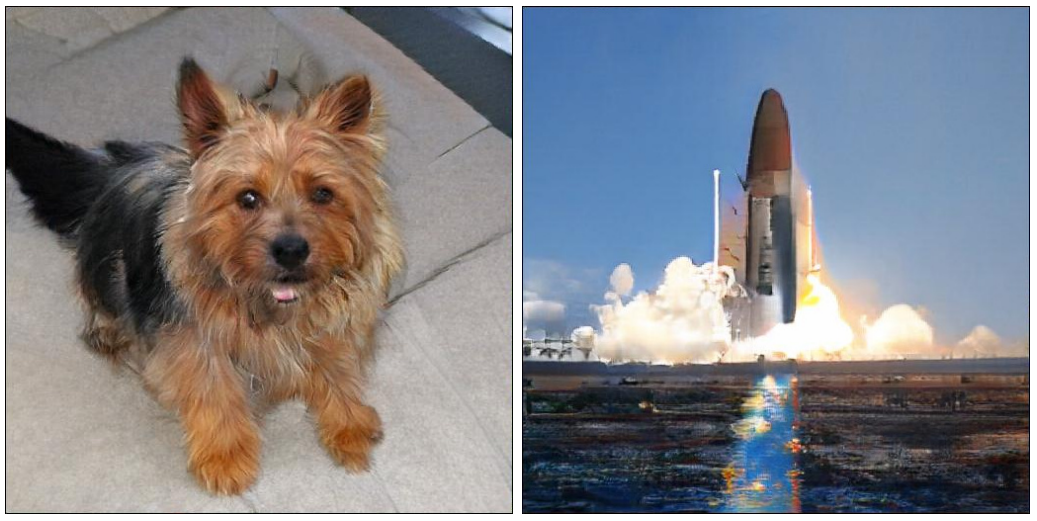
\includegraphics[width=0.55\textwidth]{graphics/biggan.png}
    \caption{Images copied from \cite{biggan}.}
    \label{fig:biggan-samples}
\end{figure}

Machine learning techniques are very powerful and have been extended problems and tasks like cancer predictions~\cite{cancer} and generating ``fake synthetic'' data~\cite{biggan}. 
Did you, \eg, notice that the images in Figure \ref{fig:biggan-samples} are ``fake''? 
The images are artificial and depict a dog and a rocket which never existed.
To generate such images, a machine learning algorithm dug through more than a million images to devise an algorithm for synthesizing ``fake'' images that look realistic. 
At the time of writing, neural networks are perhaps the most employed machine learning models due to their high performance. 
It is, \eg, a neural network that generated the images in Figure \ref{fig:biggan-samples}. 

Although neural networks are powerful and can solve a wide range of tasks, such networks also come with certain drawbacks.
First, digging through tons of data requires a lot of compute, typically on costly hardware.
For example, Some neural networks were trained for several days~\cite{alexnet, alphafold} or even weeks on \$100+ million hardware.\footnote{A very recent blog post from NVIDIA describes a generative model with 530 billion parameters trained for at least 35 days on 560 machine learning servers at an individual price of $\sim$\$200.000~\cite{nvidia-bigass-mofo}.}
Today, most major performance improvements are obtained by increasing dataset or network size (see, \eg,~\cite{gpt-3}).
Consequently, if one can derive faster machine learning algorithms, then neural networks can be improved without increasing the computational budget.
The second issue with neural networks is that the resulting algorithms that can, \eg, identify dogs and rockets in images, make predictions without any reasoning.
From such networks, it is, \eg, not straight forward how to do counterfactual reasoning about the predictions of the networks; 
similar to how we did with our own predictions above by hypothesizing about the removal of smoke and glare in the rockes image.
Even though a neural network may correctly guess, \eg, the content of an image, it is typically hard to tell \emph{why} the network guessed as it did.
Being able to tell \emph{why} could, \eg, enable us to validate the behavior of neural networks used to automatically judge humans, to ensure a fair judgement.

This thesis revolves around those two issues, \ie, how can we speed up machine learning algorithms, and how can we reason about \emph{why} particular predictions were made by neural networks? 
As a motivation for answering the latter question, we observe that when humans explain their behavior, they typically ``generate evidence'' that supports their choices.
For humans, such evidence could, \eg, be an emphasis on specific existing knowledge or a presentation of a hypothetical alternative reality for which their behavior would be different.
In any case, the evidence needs to be generated somehow.
Generating such evidence for neural network algorithms seems well aligned with the capabilities of neural networks that generate ``fake'' data, like the one generating the images in Figure \ref{fig:biggan-samples}, which are also known as generative models. 
As a consequence, we form the main hypothesis of this thesis:
%
\begin{quote}
    We hypothesize that crossing generative models with explainability can produce state-of-the-art methods for explaining neural networks. 
\end{quote}
%
This thesis sheds light on the hypothesis by considering three research questions:
\paragraph{RQ1:} \emph{How can the efficiency of machine learning algorithms be improved?}\\
If our hypothesis holds, we believe that the performance of methods for explaining neural networks will depend highly on the performance of associated generative models. 
In turn, it makes sense also to improve the performance of generative models.
Improving the training efficiency of machine learning algorithms will allow scaling up datasets or model sizes, which may yield better generative models. 
Further down-stream, better generative models potentially improve explainability methods.
In Chapter \ref{chap:nns}, we present two novel algorithms that compute already established quantities used for generative modeling, but much faster than existing algorithms.  

\paragraph{RQ2:} \emph{How can generative models be utilized for explaining neural networks?}\\
At the heart of our main hypothesis, we consider how to utilize generative models within the field of explainability.
More specifically, we consider how we can use such models to efficiently generate high-quality counterfactual examples, similar to the rocket without glare discussed above.
In Chapter \ref{chap:ecinn-main}, we present a novel method for generating such counterfactual examples efficiently.

\paragraph{RQ3:} \emph{How are methods for explaining neural networks best evaluated?}\\
To identify state-of-the-art methods, proper evaluation metrics need to be established.
In Chapter \ref{chap:evaluation}, we analyze and experimentally evaluate existing metrics for quantifying the performance of counterfactual examples before introducing two new metrics that avoid drawbacks of existing ones. 

% \section{Contributions}
% +++   0.5 pages summarizing the thesis and our contributions. 
% Contributions
% \begin{itemize} 
    % \item Improving efficiency of training with orthogonal matrices.
    % \item Allowing efficient backpropagation through FID
    % \item Method for generating counterfactuals.
    % \item Evalution of counterfactual explanations.
% \end{itemize}

% Other notes: 
% We are interested in explainaility and how to explain deep neural networks.
    % - Many methods exists. Heatmaps, transparent models, bla. We focus mainly on Counterfactual Explanations
    % - We see en immediate connection between generative models and counterfactuals and explore how to generate and evaluate counterfactual explanations from the perspective of generative models.

\chapter{Efficient Neural Network Training}\label{chap:nns}
Neural networks can be found solving a variety of problems, from classifying malignant breast tumors~\cite{cancer} to generating ``fake'' molecular compounds~\cite{chem-gan}. 
However, such remarkable performances come at a high computational cost.
For example, up to 512 specialized and costly Tensor Processing Units were used to train a single model for up to 48 hours \cite{biggan}. 
Furthermore, a current trend indicates that larger models (more compute) perform better~\cite{language-models-few-shot, scaling-matters}.
In turn, improving algorithms to allow even larger models to be trained within the same computational budget can improve performance.
Finally, we believe that as a consequence of improved performances of generative models, better methods within explainability will emerge further downstream.

This chapter presents two papers which revolve around efficient computations of central components for neural networks.
The first paper, \paperref{pap:svd}, is introduced in Section \ref{sec:svd} and was published at NeurIPS 2020 as a spotlight paper.
It introduces a fast algorithm for computing Householder products, which can be used to efficiently represent neural network weights in their Singular Value Decomposition (SVD) during training.
The second paper, \paperref{pap:fastfid}, is a manuscript presented in Section \ref{sec:fid}. 
The paper presents a new algorithm for computing the Fr\'echet Inception Distance (FID) fast for small mini-batches.
With the new algorithm, FID can be optimized directly as a part of a loss function, which, prior to our work, was practically infeasible. 
Finally, Section \ref{sec:nn-discussion} is devoted to discussing the impacts of the two papers. 

\section[What if Neural Networks had SVDs?]{What if Neural Networks had SVDs?\contribution{pap:svd}} \label{sec:svd}
% +++ 1 page on motivating the problem, e.g., with a couple of examples of where it makes sense.
This section gives a brief introduction to the problem that the presented algorithm solves and the high-level contributions of the paper, before putting it into context of related work. 
Successively, applications where our algorithm improves computational efficiency are presented.
Finally, further details about the algorithm ends this section.
% TODO Make sure introduction is right.

% 1. Present at a high level what FastH does. Not the technical part but just the result.
During training, many neural networks need to perform time-consuming operations like, \eg, matrix inversions, spectral normalization, and determinant computations of weight matrices~\cite{nice, realnvp, glow, sngan}.
A standard implementation of, \eg, the matrix determinant $det(W)$ for $W\in\mathbb{R}^{d\times d}$ typically takes $O(d^3)$ time, which for a large $d$ may constitute a bottleneck in the overall training time. 
As such, finding a way to speed up determinant computations will allow using larger weight matrices within the same computational budget, thus obtaining larger neural networks.
One way to decrease computation time is to represent weights $W$ in their SVD, $W = U\Sigma V^\intercal$ where $U, V \in \mathbb{R}^{d\times d}$ are orthogonal, \ie, $U^{-1} = U^\intercal$ and $V^{-1}= V^\intercal$, and $\Sigma\in \mathbb{R}^{d\times d}$ is a diagonal matrix. 
In such decomposition, computing the determinant of $W$ takes just $O(d)$ time, $det(W) = det(U\Sigma V^\intercal) = det(U)det(\Sigma)det(V^\intercal) = 1\cdot \prod_{i=1}^d \Sigma_{i,i} \cdot 1$.
It is, however, not straightforward to optimize $U$ and $V$ in such representation.
An immediate issue is that doing gradient updates on $U$ and $V$ directly is not guaranteed to maintain the orthogonality of $U$ and $V$.
\citet{sequential} propose to parametrize each orthogonal matrix as a composition of $d$ Householder matrices $H_i$ that are stored as $d$-dimensional vector $v_i$, to circumvent this issue:
\begin{equation}\label{eq:hh-decomposition}
    V = \prod_{i=1}^d H_i, \qquad H_i = I - 2\frac{v_i v_i^\intercal}{\| v_i \|_2^2}.
\end{equation}
In Equation \ref{eq:hh-decomposition}, each $H_i$ is orthogonal, which makes $V$ orthogonal as well. 
Furthermore, any $d$-dimensional orthogonal matrix can be represented by such decomposition~\cite{qrhh}. 
The parametrization makes gradient descent possible by preserving the orthogonality of $U$ and $V$ during optimizations, while the matrix product $WX = U \Sigma V^\intercal X$ can be evaluated in $O(d^2m)$ for a mini-batch of $m$ samples $X\in\mathbb{R}^{d\times m}$, similar to regular matrix multiplication. 
There is, however, a catch.
The decomposition is inherently sequential. 
That is, to evaluate $WX$, one must compute $O(d)$ sequential matrix-vector operations, which is ill-fit for GPUs.\footnote{We distinguish matrix-vector and matrix-matrix operations because GPUs are highly parallel and much more efficient on matrix-matrix operations. Matrix-matrix operations are thus preferred.}
Specifically, for both $U$ and $V$, $H_1(H_2(...(H_dX) ...))$ is computed sequentially, as indicated by the parenthesis.
We will denote this approach as the ``sequential algorithm.'' 
As most machine learning models today are trained on highly parallel hardware like GPUs, sequential algorithms are typically slow compared to parallel algorithms.

\citet{sequential} notice that the sequential algorithm is slow. 
As a consequence, they suggest an additional algorithm based on matrix-matrix products, which is more parallel and thus a better fit for GPUs. 
The algorithm first constructs the orthogonal matrices $U$ and $V$ by multiplying together $H_1, ..., H_d$, before evaluating $WX = U\Sigma V^\intercal X$.
Without any further utilization of the Householder structure in Equation \eqref{eq:hh-decomposition}, such algorithm takes $O(d^3)$ time and still entails $O(d)$ sequential steps.
From this point on, we denote this algorithm as the ``parallel algorithm.''
Due to increased parallelization, the parallel algorithm is faster than the sequential in practice, even though it is less efficient asymptotically.
Even if the Householder matrices are computed in a tree structure $U = (...((H_1H_2)(H_3H_4))...(H_{d-1}H_d)...)$ to obtain $O(\log d)$ sequential steps, the asymptotic running time of multiplying the higher level $d\times d$ matrices will entail an $O(d^3\lg d)$ running time, which is not even as fast as computing the SVD in $O(d^3)$ time in the first place.
This raises an intriguing question; can we compute $WX$ in the fast asymptotic running time $O(d^2m)$ with less than the $O(d)$ sequential work?  
% multiplies the Householder matrices together first, which is more parallel, but takes $O(d^3)$ time, as fast as computing the $SVD$ in the first place, because at least $d/2$ $d\times d$ matrices must be multiplied together.

\paragraph{Contributions.} In \paperref{pap:svd}, we introduce a GPU friendly algorithm FastH, which computes the same Householder product, obtains the fast asymptotic running time $O(d^2m)$, and requires only $O(t + d/t)$ sequential matrix-matrix operations for an adjustable group size $t$, as compared to $O(d)$ sequential matrix-vector computations used by the sequential algorithm.
In practice, we find that FastH is up to 27 times faster than the sequential algorithm and six times faster than the parallel. 
Before presenting the details of the FastH algorithm in Section \ref{sec:fasth}, applications of representing weight matrices in their SVD and related work are described next.

\subsection{Applications}\label{sec:fasth-applications}
Besides the determinant computations, which we have already mentioned, we describe three additional applications for which parametrizing weight matrices by their SVDs has advantages in terms of computational speed-ups.

The first example is the matrix inverse. 
Inverting a $d\times d$ matrix generally takes $O(d^3)$ time.
With the SVD, the matrix inverse can be computed as follows:
\begin{equation}\label{eq:svd-inverse}
    W^{-1} = (U\Sigma V^\intercal)^{-1} = (V^\intercal)^{-1}\Sigma^{-1}U^{-1} = V \Sigma^{-1} U^\intercal.
\end{equation}
From Equation \eqref{eq:svd-inverse}, inverting $W$ requires only a diagonal inverse and two transposes.
% we see that transposing $U$ and $V$, and inverting the diagonal matrix $\Sigma$ is enough.
In the Householder representation shown in Equation \eqref{eq:hh-decomposition}, multiplying with the transpose of $U$ or $V$ corresponds to reversing the order of the Householder matrices.
In turn, the transpose operation takes constant time. 
Inverting a diagonal matrix takes $O(d)$ time. 
Consequently, the inverse takes $O(d)$ time rather than $O(d^3)$.

The second example is weight decay, which is arguably one of the most established regularizers of neural networks.
The squared Frobenius norm has the property that it can be computed as the sum of squared singular values, \ie, $\|W\|_F^2 = \sum_{i,j=1}^d W_{i,j}^2 = \sum_{i=1}^d \Sigma_{ii}^2$.
Therefore, when we can read off the diagonal of $\Sigma$ directly, we can compute weight decay in $O(d)$ time instead of the $O(d^2)$ time it takes to compute the square of all entries in $W$.
Additionally, some works utilize the nuclear norm, which is the sum of singular values $\|W\|_\ast = \sum_{i=1}^d \Sigma_{i,i}$~\cite{nuclear-norm-regularizer, nuclear-norm-regularizer2}. 
In contrast to the Frobenius norm, the nuclear norm requires explicitly computing the SVD in $O(d^3)$ time at each training step.
Although not straight forward to apply to the mentioned work due to further optimization details, such norm can be computed in $O(d)$ time if $\Sigma$ is known.
%to optimize $U$ and $V$ in the mentioned work due to additional training details, such norm could again be computed in $O(d)$ time if $\Sigma$ was known. 

The third and final application is spectral normalization, which is used to train generative adversarial networks~\cite{sngan, wgan} and make neural networks more robust against adversarial attacks~\cite{spectral-norm-robustness}. 
Spectral normalization constrains the largest singular value of $W$ to be one, \ie, $W = W / \max_{i}(\Sigma_{i,i})$. 
As discussed, computing the SVD to find $\Sigma$, and thus $\max_i(\Sigma_{i,i})$, takes $O(d^3)$ time, which is typically too slow in practice.
Related work often circumvents the high computational cost by clipping the weights~\cite{wgan} or approximating the largest singular value through the power iteration algorithm~\cite{sngan, spectral-norm-robustness}.
The approximation takes $O(d^2r)$ time, where the approximation error decreases with a larger $r$.
If $W$ is represented in its SVD, identifying the exact largest singular value can be done in $O(d)$ time by simply inspecting $\Sigma$. 

\subsection{Related Work}
Here, we have categorized related work into three levels.
At the highest level, there exist works that use the SVD or more general tensor decompositions for training neural networks.
At an intermediate level, orthogonal matrices have also been employed in neural networks for different reasons.
Finally, at the lowest level, various methods for enabling the optimization of orthogonal matrices also exist.

As is well known, the SVD is closely tied to the dimensionality reduction method Principal Component Analysis, as the columns of $U\Sigma$ are the principal components of a data matrix $X = U \Sigma V^\intercal$.
After training a neural network, a natural way to compress the network to get a faster ``low-rank approximation'' of the network is to use only the first $k$ principal components of each weight matrix.
To circumvent training large networks before compressing them, this idea has been extended in multiple ways.
For example, \citet{training-svd-regularized} propose to optimize weights of both dense layers and (reshaped) convolutional layers in their SVD by regularizing $U$ and $V$ to be approximately orthogonal through loss terms like $\|UU^\intercal-I\|_F^2$.
\citet{convolution-tensor-decomposition} also propose a multi-linear tensor decomposition of convolutional filters to achieve efficient low-rank convolutional kernels that can be trained in an end-to-end fashion.

% Tensor decompositions / SVD / PCA.
% - \cite{training-svd-regularized} strin in the SVD with \|UU^T - I\|_F^2 regularization.
% - Alekos work on end-to-end learnable tensor decompositions \cite{convolution-tensor-decomposition} trains low rank multilinear convolutions. 
An area of research where orthogonal matrices are of high importance and often utilized is within recurrent neural networks (RNN).
Given a long sequence of samples $x_1, ..., x_t\in\mathbb{R}^{m}$, recurrent neural networks are applied over and over again along the sequence of samples with the output from the previous sample as a part of the input, \ie, $f(x_t, ...f(x2, f(x_1, 0)) ... )$ where $f$ has the structure $f(x, z) = \sigma( Vx + Wz) )$ with $V\in \mathbb{d\times m}$, $W\in\mathbb{R}^{d\times d}$, and $\sigma$ being some point-wise non-linearity~\cite{urnn}.
For such computations, gradient computations become very ``long,'' which can result in vanishing or exploding gradients if $W$ and $\sigma$ are not norm preserving.
Orthogonal matrices are norm preserving, \ie, $\|Ux\|_2 = \|x\|_2$, and constitute central building blocks for avoiding exploding (or vanishing) gradients.
To the best of our knowledge, \citet{urnn} were the first to parametrize orthogonal matrices for RNNs through a product of cleverly chosen low memory footprint and efficient complex unitary matrices, such that $Wx_i$ can be evaluated in $O(d \log d)$ time.
However, the resulting orthogonal matrices are limited in what they can express. 
Informally, this is due to a limited $O(d)$ free parameters of the complex matrices.
Successively, \citet{hh-rnn} proposed to instead parametrize the orthogonal matrix with $O(d)$ Householder matrices to parametrize the $W$s in RNNs with $O(d^2)$ parameters. 
\citet{sequential} further utilize a Householder parametrization to form an SVD of $W$ where the singular values are restricted to be close to one, \ie, $\Sigma_{i,i} \in [1\pm\varepsilon]$ for $\varepsilon > 0$. 
As described, \cite{sequential} presents both a sequential and a parallel algorithm for evaluating the Householder parametrization.
For an input $X\in\mathbb{R}^{d\times m}$, evaluating $WX$ sequentially has an $O(d^2m)$ time complexity but is slow in practice. 
The parallel algorithm is faster in practice but has an $O(d^3)$ time complexity. 
FastH is a new algorithm that shares the fast $O(d^2m)$ time complexity while being fast in practice; 
FastH is up to six times faster than the parallel algorithm.
It should also be mentioned that concurrent with \paperref{pap:svd}, \citet{cwy-dec} also notice the gap between the sequential and parallel algorithm and present a different parallel algorithm for evaluating Householder products from a related CWY decomposition, which relies on matrix inversion that takes $O(d^3)$ time.

Another area where orthogonal matrices are employed is in Normalizing Flows where, \eg, determinant computations of weight matrices can be needed~\cite{glow}.
As a way of parametrizing square matrices such that determinants can be computed efficiently, \citet{emerging} propose to utilize the QR decomposition $W = QR$, where $Q\in\mathbb{R}^{d\times d}$ is an orthogonal matrix parametrized by the Householder decomposition described in Equation \eqref{eq:hh-decomposition} and $R\in\mathbb{R}^{d\times d}$ is a triangular matrix.
In such decomposition, the determinant computation has $O(d)$ time complexity because $det(W) = det(Q) \cdot det(R) =1 \cdot  \prod_{i=1}^d R_{i,i}$. 
In \cite{emerging}, they employ a sequential algorithm for the householder decomposition and could gain a practical speed-up by using FastH. 

Finally, there also exist other ways of parametrizing orthogonal matrices.
Skew symmetric matrices $W^\intercal = -W$ has the property that for both the matrix exponential $Q = e^W$ and the Cayley transform $Q=(I-W)(I+W)^{-1}$, $Q$ is orthogonal~\cite{matrixexp1}. 
However, \citet{matrixexp1} approximate matrix exponentials with an algorithm that run in $O(d^3)$ time.  
As a consequence, such exponentials are typically used in RNNs where the input sequence lengths $s$ is much larger than the hidden state dimensionality $d$.
For such situations, computing the matrix exponentials becomes asymptotically faster than evaluating the RNN on the whole sequence, \ie, $O(d^3) < O(d^2s)$ when $d \ll s$.

\subsection{FastH}\label{sec:fasth}
From the observation that there is a gap between the slow (in practice) $O(d^2m)$ sequential algorithm and the faster parallel $O(d^3)$ algorithm from \cite{sequential}, we raised the following question.

\begin{problem}
    Given $X\in \mathbb{R}^{d\times m}$ and $v_1, ..., v_d \in \mathbb{R}^{d}$, can we evaluate the product $\left[ \prod_{i=1}^d I-2\frac{v_iv_i^\intercal}{\|v_i\|_2^2}\right]X = \left[\prod_{i=1}^d H_i\right]X$ in $O(d^2m)$ time with less than $O(d)$ sequential matrix-matrix operations?
\end{problem}

The short answer i ``yes,'' FastH computes the Householder product in $O(d^2m)$ time while using just $O(d/t) + t$ sequential operations, where $t$ is an intermediate result size, as presented next.

FastH increases parallelism by grouping Householder products into intermediate results $G_j$ representing products of $t$ Householder matrices in a convenient decomposition which allows computing $G_jX$ fast. 
The core insight needed to form our algorithm is a result dating back to 1987~\cite{wydec}.
We rephrase the result in our notation in Lemma \ref{lem:wydec}:

\begin{lemma}\label{lem:wydec}
For any $t$ Householder matrices $H_1,...,H_t$, there exists $W,Y\in \mathbb{R}^{d\times t}$ st. 
$I-WY^\intercal = H_1 \cdots H_t$. 
Computing $W$ and $Y$ takes $O(dt^2)$ time and $t$ sequential matrix-matrix multiplications. 
\end{lemma}

FastH computes the Householder product $H_1H_2...H_dX$ through two steps.

% \paragraph{Step 1.}
\begin{description}
	\item[Step 1:] The product is split into $d/t$ groups, for which the decomposition from Lemma \ref{lem:wydec} of each group is computed in parallel.
\newcommand{\veq}{\mathrel{\rotatebox{90}{$=$}}}
\begin{equation}
    \begin{matrix}
        H_1...H_t & H_{t+1}...H_{2t} & ... & H_{d-t+1}...H_d \\
        \veq  & \veq & ... & \veq\\
        G_1 = I -W_1Y_1^\intercal & G_2 = I - W_2Y_2^\intercal & ... & G_{d/t} = I - W_{d/t}Y_{d/t}^\intercal
    \end{matrix}.
\end{equation}
% \paragraph{Step 2.}
\item[Step 2:] From the decompositions, $G1(G2(...(G_{d/t}X)...))$ is computed sequentially by multiplying $X$ on each decomposition from right to left, as indicated by the parenthesis.
\end{description}

With Lemma \ref{lem:wydec} at hand, we analyze the time complexity of FastH.
In step 1, there are $d/t$ groups requiring an $O(dt^2)$ computation each, yielding an $O(d^2t)$ time complexity.
In step 2, there are $d/t$ groups, where two matrices of size $t\times d$ are multiplied with the input of size $d \times m$ in $O(tdm)$ time, leading to an $O(d/t \cdot tdm) = O(d^2m)$ total time complexity.
As a result, FastH shares the $O(d^2m)$ running time with the sequential algorithm from \cite{sequential}.

To analyze how many sequential operations are needed for FastH, we again consider the two steps.
According to Lemma \ref{lem:wydec}, step one needs $O(t)$ sequential matrix-matrix operations.
Step 2 needs to multiply $X$ with each group sequentially, yielding $O(d/t)$ additional sequential matrix-matrix operations.
This leads to a total of $O(t + d/t)$ sequential matrix-matrix operations, as compared to the $O(d)$ sequential matrix-vector operations in \cite{sequential}. 

We note that some details have been left out in the above description of FastH. 
In \paperref{pap:svd}, we, \eg, present an algorithm for performing gradient computations as efficient as the ``forward computations.''
We also provide CUDA code, such that our algorithm can run efficiently on GPUs.

\section[Backpropagating through Fr\'echet Inception Distance]{Backpropagating through Fr\'echet Inception Distance\contribution{pap:fastfid}} \label{sec:fid}
% +++ 1 page on motivating the problem.
% - FID is currently used primarily to evaluate generative models.
% - If it is such a nice metric, shouldn't we be able to train with it directly?
At the time of writing, unsupervised generative modeling is a vibrant field of research.
Informally, generative modeling aims at approximating a data distribution to generate \emph{fake} data that is likely to stem from the data distribution.
Within this area, deep neural networks have been employed as building blocks for various types of generative models.
To name but a few, Variational Auto-encoders (VAEs)~\cite{vae}, Generative Adversarial Networks (GANs)~\cite{gans}, Normalizing Flows~\cite{nice}, and Score-based generative models~\cite{sgm-stochastic-differential-equations} are some techniques based on neural networks.

Not all types of generative models are based on likelihood, so a direct comparison of their performance is not trivial.
Perhaps the most conventional way of evaluating generative models for images across model types is the Fr\'echet Inception Distance (FID)~\cite{fid, fid-comparison}. 
The FID approximates how distant two distributions are, given samples from the two distributions. 
In the context of generative models, the two distributions are the \emph{real} data distribution $p(x)$ and the distribution of the \emph{fake} data $q(x)$ from the generative model.
As the generative model tries to approximate the sampling process of real data distribution, a lower FID is better.
We hypothesize that explicitly minimizing FID as a loss will yield a better validation FID.
The purpose of \paperref{pap:fastfid} is to test this hypothesis.
Computing FID at every training step with the original algorithm is computationally too expensive to be used in practice.
With our new algorithm FastFID, the FID can be computed fast enough to be used as a loss function. 

To compute the FID, one first draws $n$ real samples $r_1, r_2, ..., r_n \sim p(x)$ and $m$ fake samples $f_1, f_2, ..., f_m\sim q(x)$.
Successively, all $r_i$ and $f_i$ are encoded by computing the activations of the final hidden layer of the pretrained Inception-V3 network~\cite{inceptionv3}, $A(r_i)$, $A(f_i)$.
Two multivariate normal distributions are then formed from the statistics of the encodings, $\mathcal{N}(\mu_r, \Sigma_r)$, $\mathcal{N}(\mu_f, \Sigma_f)$.
Finally, the FID is the Fr\'echet distance (also known as the Wasserstein-2 distance) between the two normal distributions:
\begin{equation}\label{eq:fid}
    \operatorname{FID}(\mu_r, \Sigma_r, \mu_f, \Sigma_f) = \| \mu_r - \mu_f \|_2^2 + tr(\Sigma_r + \Sigma_f) - 2\cdot tr(\sqrt{\Sigma_r \Sigma_f}).
\end{equation}
\citet{fid} demonstrate how the FID correlate well with both human judgement and increasing disturbance, \eg, by adding increasing levels of noise. 

When computing the FID, only $\mu_f$ and $\Sigma_f$ change across different generative models.
As such, much computation can be cut by computing encodings $A(r_i)$ and successively $\mu_r, \Sigma_r$ just once.
In fact, \citet{fid} even share precomputed statistics for five popular datasets.\footnote{\url{https://github.com/bioinf-jku/TTUR}}
But even then, the computational complexity of the FID is $O(d^3 + d^2m)$, where the first term stems from the matrix square root $\sqrt{\Sigma_r\Sigma_f}$ and the second term comes from computing $\Sigma_f$ from the encodings.

To obtain a robust result, \citet{fid} compute the FID based on $n=m=10 000$ samples during training.
It is time-consuming to both encode $10 000$ images and to successively compute the FID.
For example, on an NVIDIA RTX 2080 Ti GPU, it takes roughly $20s$ to compute the FID; around $10s$ is spent computing fake encodings and $10s$ is spent computing $\sqrt{\Sigma_r\Sigma_2}$.
We hypothesize that such heavy computations have kept researchers from actively using the FID as a training loss. 
This hypothesis raises an interesting question. 
Is it possible to compute the FID fast enough for it to be used as a training loss?

\paragraph{Contributions.} 
In \paperref{pap:fastfid}, we introduce FastFID; an algorithm which computes the FID on mini-batches (few fake samples, $m \ll d$) in $O(d^2m + m^3)$ time. 
FastFID is up to three orders of magnitudes faster and has at least three orders of magnitude less numerical error than the original algorithm.
We demonstrate how the algorithm is fast enough to be used for explicitly training GANs with FID as a loss function, resulting in a better validation FID. 
We further establish evidence indicating that using the FID as a loss function improves the quality of generated fake images.
For example, images of a dog get new semantic features like eyes and ears. 

\subsection{Related Work}
While there exist many publications, which use FID to benchmark generative models~\cite{fid-comparison, saganfid, biggan, dcgan}, we know of no publications which use the FID as a loss function.
Neither do we know of any prior work, which reduces the computational complexity of the FID.
As such, related work is relatively sparse.
There does, however, exist a couple of ways to approximate the FID.\footnote{\label{fn:tf}\url{https://github.com/tensorflow/tensorflow/blob/00fad90125b18b80fe054de1055770cfb8fe4ba3/tensorflow/contrib/gan/python/eval/python/classifier_metrics_impl.py}}
For example, one can ignore the second moments of the normal distributions and only compute $\|\mu_r-\mu_f\|_2^2$ (\href{https://github.com/tensorflow/tensorflow/blob/00fad90125b18b80fe054de1055770cfb8fe4ba3/tensorflow/contrib/gan/python/eval/python/classifier_metrics_impl.py#L525}{line 525} in \footnoteref{fn:tf}) in $O(dm)$ time for a mini-batch.
Similarly, \citet{approximate-fid} propose to train a GAN by only considering the mean and the diagonal entries of the covariance matrices, also in $O(dm)$ time (previously also employed in \href{https://github.com/tensorflow/tensorflow/blob/00fad90125b18b80fe054de1055770cfb8fe4ba3/tensorflow/contrib/gan/python/eval/python/classifier_metrics_impl.py#L582}{line 582} in \footnoteref{fn:tf}).
Finally, \citet{fid-approx} propose an algorithm for approximating the matrix square root with a variant of Newton's method for root finding, which provide an approximation that is much faster than the original implementation of FID.

% Furthermore, they state that $FID$ should be computed for at least $2048$ samples to ensure that $\Sigma_r\Sigma_f$ has full rank, which avoids complex numbers and \verb^NaN^s when computing $tr(\sqrt{\Sigma_r\Sigma_f})$ directly.
% However, as we will demonstrate shortly, with our proposed algorithm, we can compute the trace without explicitly computing the matrix square root.
% As a consequence, we can compute the quantity for even less samples without this issue occuring.

\subsection{Fast Fr\'echet Inception Distance} 
To describe how FastFID works, we first highlight how the previous algorithm from \cite{fid} computes the FID before describing FastFID in details.

\paragraph{The previous algorithm.} As described above, there are two bottlenecks in FID computations, computing the encodings and computing the trace of the matrix square root.
% The first bottleneck can be circumvented by precomputing statistics for the real samples.
Precomputing statistics for the real samples can circumvent the first bottleneck.
Furthermore, for a mini-batch, we would only need to compute encodings for $m \ll d$ fake samples.
These two improvements jointly cut the overall computational complexity for computing statistics from $O(d^2(m+n))$ to $O(d^2m)$.
As an example, if we use precomputed statistics and reduce $m$ from $10 000$ to $128$, this reduces the time it takes to encode samples from roughly $10s$ to $0.1s$ on our machine.
This is a known improvement that was already done by~\cite{fid}.

In \paperref{pap:fastfid}, we contribute with a large speed-up for the second bottleneck.
Originally, $tr( \sqrt{\Sigma_r \Sigma_f} )$ was computed by first constructing $\Sigma_r \Sigma_f$ to successively compute the matrix square root and the trace.

The matrix square root is found by first computing the Schur decomposition:
\begin{equation}\label{eq:schur}
    \Sigma_r\Sigma_f = QVQ^\intercal, \qquad \text{with }Q^\intercal = Q^{-1}\text{ and triangular }V.
\end{equation}
Given the decomposition, finding the square root amounts to computing a triangular matrix $U$ such that $U^2 = V$, which implies that $\sqrt{\Sigma_r \Sigma_f} = QUQ^\intercal$ since $(QUQ^\intercal)^2 = QU^2Q^\intercal = QVQ^\intercal = \Sigma_r\Sigma_f$.
Now recall that the trace of a matrix is equal to the sum of the eigenvalues.
For the sake of readability, we state it as a lemma here:
\begin{lemma}\label{lem:trase-eigenvalues}
    For a matrix $A\in\mathbb{R}^{d\times d}$ with eigenvalues $\lambda_i(A)$, $tr(A) = \sum_{i=1}^{d}\lambda_i(A)$~\cite{matrix-cookbook}.
\end{lemma}
As $U$ contains the eigenvalues of $\sqrt{\Sigma_r\Sigma_f}$ on the diagonal, it is sufficient to compute the trace of $U$ in $O(d)$ time, $tr(\sqrt{\Sigma_r\Sigma_f}) = tr(U)$.
Computing both the Schur decomposition and $U$ takes $O(d^3)$ time, which is also to computational complexity of the whole computation of the trace of the matrix square root.
In turn, the total time complexity of the previous algorithm is $O(d^3 + d^2m)$.

\paragraph{FastFID.}
Consider the following lemma.
\begin{lemma}\label{lem:product-eig}
    For two matrices $A, B$, the eigenvalues of $AB$ and $BA$ are the same if the two products are both square matrices~\cite{low-rank-eigenvalue-problem}.
\end{lemma}
To compute the trace of the matrix square root faster, we utilize both Lemma \ref{lem:trase-eigenvalues} and Lemma \ref{lem:product-eig} to construct a matrix $M\in \mathbb{R}^{m\times m}$ which is much smaller than $\Sigma_r\Sigma_f$. 
In turn, the eigenvalues and thus the trace is faster to compute.
Specifically, for a mini-batch, \eg, with $m=128$ samples, computing the eigenvalues of a $m\times m$ matrix in $O(m^3)$ time is much faster than computing the Schur decomposition above in $O(d^3)$ time, as $d$ is typically $2048$.
Below, we describe the details of our algorithm. 

With $\mathbb{1}_k \in \mathbb{R}^k$ being the all-ones vector, define centered data matrices $X_r\in\mathbb{R}^{d\times n}$ and $X_f\in \mathbb{R}^{d\times m}$ as the real and fake encodings over the columns, respectively:
\begin{equation}
    X_r = \left[
        \begin{matrix}
            | & & |\\
            A(r_1) & ... & A(r_n)\\
            | & & |
        \end{matrix}
    \right] - \mu_r\mathbb{1}_n^\intercal \qquad
    X_f = \left[
        \begin{matrix}
            | & & |\\
            A(f_1) & ... & A(f_m)\\
            | & & |
        \end{matrix} 
    \right] - \mu_f\mathbb{1}_m^\intercal.
\end{equation} 
Sample covariance matrices can then be computed as a product of such matrices:
\begin{align}
    \Sigma_r = C_rC_r^\intercal\text{,}\quad \Sigma_f=C_fC_f^\intercal\quad\text{ where }\quad & C_r = \frac{1}{\sqrt{n-1}}X_r\\
    \text{ and }\quad & C_f = \frac{1}{\sqrt{m-1}}X_f.
\end{align}

A corollary of Lemma \ref{lem:trase-eigenvalues} is that $tr(\sqrt{A}) = \sum_{i=1}^d \sqrt{\lambda_i(A)}$.
In turn, $tr(\sqrt{\Sigma_r\Sigma_f}) = \sum_{i=1}^d \sqrt{\lambda_i(\Sigma_r\Sigma_f) }$.
However, computing the eigenvalues of $\Sigma_r\Sigma_f$ still takes $O(d^3)$ time.
Due to Lemma \ref{lem:product-eig}, we can compute the eigenvalues of the $m\times m$ matrix $C_f^\intercal C_rC_r^\intercal C_f$ in $O(m^3)$ time instead of the $d\times d$ matrix $C_rC_r^\intercal C_fC_f^\intercal$.
Specifically, FastFID computes the trace of the matrix square root in $O(m^3 + d^2m)$ time by avoiding constructing $\Sigma_r\Sigma_f$ explicitly:
\begin{equation}\label{eq:fastfid}
   tr( \sqrt{\Sigma_r\Sigma_f}) = \sum_{i=1}^{d-1}\sqrt{\lambda_i(C_rC_r^\intercal C_fC_f^\intercal)} = \sum_{i=1}^{m-1} \sqrt{\lambda_i(C_f^\intercal C_rC_r^\intercal C_f)}
\end{equation}
Note that the $d^2m$-term in the time complexity stems from computing $(C_f^\intercal C_r)(C_r^\intercal C_f)$.

We note that for simplicity, some details have been hidden in this description.
For example, in \paperref{pap:fastfid}, we compare numerical errors between the previous algorithm and FastFID.
As a consequence, we need the two algorithms to compute exactly the same quantity.
The matrix square root is not unique, so we need to apply the absolute value $|\sqrt{\lambda_i(C_f^\intercal C_rC_r^\intercal C_f)}|$ in Equation \eqref{eq:fastfid} to comply with \verb^scipy.linalg.sqrtm^.
Furthermore, the FID can also be extended to other types of data than images.
For example, the same metric has also been applied to chemicals~\cite{fcd} by encoding data with another neural network.
FastFID also extends to such applications.

Apart from the theoretical contributions described here, we perform multiple experiments.
Naturally, we test how fast FastFID is in practice.
We find that for sufficiently small mini-batches (small $m$), FastFID can be up to three orders of magnitudes faster than the previous algorithm.
We also demonstrate that FastFID is fast enough to use FID as a training loss.
Across three different GANs on three different datasets of increasing complexity, we demonstrate that adding FID as an additional loss term improves the validation FID.
Finally, we attempt to determine whether using FID as a loss function yields better images.
From our experiments, we find that fine-tuning a generator of a pre-trained GAN, solely using the FID as a loss, yields images with more semantic features like beaks, ears and eyes.
As such, we conclude that using FID as a loss function has great potentials in terms of improving the quality of generative models.
 
 
\section{Discussion}\label{sec:nn-discussion}
% In the two papers, we introduce algorithms to speed up and improve training of neural networks.
% We believe that such improvements can have positive impacts further down stream, when considering explainability, as they can both be used to improve generative models.

With the FastH algorithm in \paperref{pap:svd}, we have introduced an algorithm that can be plugged directly into essential layers of Normalizing Flows to improve efficiency.
Consequently, using FastH enables researchers to train larger models within the same time budget.
FastH can also be used in GANs, where weight matrices can be parametrized in their SVD to allow efficient normalization of such weights.
As scaling models up tends to yield better performances, we are optimistic that FastH can contribute to better-performing models.

There are, however, some caveats. 
For example, using the less efficient matrix exponential or the Cayley map to parametrize orthogonal matrices comes with the theoretical guarantee that no spurious minima will be introduced to the training dynamics~\cite{matrixexp1}.  
Although Householder products are expressive, such guarantees are currently not known about the Householder products. 
As such, researchers may prefer theoretical guarantees to speed, which can potentially limit the applicability of FastH.

With the FastFID algorithm, we have enabled researchers across all types of gradient-based generative models to include the FID as an additional loss term, which can potentially improve the quality of the generated ``fake'' data.
As such, we believe that the presented work constitutes an important step towards better performing generative models.
We that such improvements can also improve the quality of explanations further downstream. 

As is described in \paperref{pap:fastfid}, we tried extending the original log-likelihood loss of a Normalizing Flow with an additional FID term.
We found that the extension leads the Normalizing Flow to ``fooling'' the FID loss by adding unrealistic artifacts to the generated images. 
Backed by our experiment, we hypothesize that the discriminators of GANs ``detect'' such artifacts and penalize them through the GAN loss, which is why such artifacts does not occur in fake samples from GANs trained with the additional FID term.
This observation leaves best practices for applying the FID to generative models without discriminators as an open problem.

As the main hypothesis of this thesis is that crossing research within explanations for neural networks with research within generative modeling has high potential; we continue to believe that both the presented algorithms can improve techniques within explainability further down-stream.
The next chapter is devoted to presenting approaches for using generative models as central components for generating counterfactual examples for neural networks. 

% % % % % % % % % % % % % % % % % % % % % % % % % % % % % % % % %
% COUNTERFACTUAL EXAMPLES                                       %
% % % % % % % % % % % % % % % % % % % % % % % % % % % % % % % % %
\chapter{Counterfactual Examples} \label{chap:ecinn-main}
% +++ 1 page of introduction

% 1. Neural Networks increasingly popular. For image classification, they even surpass human performance on some tasks.
On many machine learning tasks, deep neural networks obtain state-of-the-art performances, sometimes even surpassing human performance~\cite{noisyStudent}.
For such networks to be applicable in practice, it is often critical that humans understand their behavior to be able to validate, justify, and reason about their predictions. 
The field of explainable machine learning aims at developing methods that provide such understanding.
% 2. This carries a need for ways to explain neural networks. We try to answer questions like "What information in the input made the network predict a certain output?", "What is the general behavior of the network?", and "How can I change the input in a meaningful way such that the predicted outcome changes?"
Methods typically answer questions like ``For input X, what information in X made the model predict class Y?,''  ``What general patterns is the model looking for?,'' and ``How can I meaningfully change the input such that the predicted outcome changes?.'' 
There exist many methods for answering such questions. 
%    Answering such questions gives a greater insight into the networks and allows users to get a deeper understanding of their behavior. It also allows identifying biases in the models and better understanding research from analyzing outcomes of models on research specific data. 
% 3. Lots of methods exists. Some methods produces heatmaps, which identify salient input features, which were inportant for the predictions. Others produces maps of inputs which maximized activations of different neurons to detect what characteristics different neurons are looking for. 
Methods producing heatmaps typically answer the first question \cite{lrp}, while methods identifying inputs that maximize specific neurons answer the second question \cite{carter2019activation}. 
The third question is related to counterfactual examples, which is the main focus of this chapter.
%, which relates to the main focus of this chapter, is associated with counterfactual examples.
Counterfactual examples identify how to alter inputs such that their predicted classes change.

% 4. A perticular type of explanations are counterfactual examples.
%   - Give a couple of examples of how they are useful and how they might be applied to different applications / fields of research.
A typical example of a counterfactual example is when a loan applicant is told that to get the loan, the applicant needs to earn another 200 EUR per month or have 10 000 EUR more in savings.
Such adjustments can be seen as a counterfactual examples, as the applicant is shown ``alternative realities'' where the loan is granted.
%told that had the salary not been $X$ but $X+200$ and savings not been $Y$, but $Y+200$, then the loan would have been granted. 
To further illustrate the future prospects of counterfactual examples, suppose you have an accurate model that predicts side effects from molecular compounds.
For such a model, counterfactual examples could, \eg, be similar molecular compounds but without certain side effects~\cite{carter2017using, moses}.
Having access to such counterfactuals could potentially speed up drug development and improve the effectiveness of the drugs by guiding research towards drugs without side effects.
Similar benefits could be found in other data-driven research fields.
For example, it would be possible to analyze autonomous vehicles misinterpreting their video feed or surveillance systems picking out candidates for screening~\cite{goyal19a}. 
In turn, counterfactual examples can potentially be of high value for data-driven research and many practical applications. 

% 5. The more formal definition:
%   - Give formal definition from causal structural models
%   - Adapt definition to non-structural data and neural networks.
%   - Give an example of a counterfactual example which conforms to the definition in terms of images.
Counterfactual examples were originally introduced with causal structural models, where variables are related in causal graphs~\cite{pearl2015a}.
In such a setup, it is possible to estimate probabilities of variable outcomes, given specific changes to other variables.
For most machine learning models, it is, however, not the case that variables are related in structural causal models.
In such cases, a more relaxed problem is studied, where we consider counterfactuals of the following type: 
\begin{problem}\label{def:dl-counterfactual}
    \textbf{None-causal counterfactual:} A none-causal counterfactual question seeks what should be changed to obtain a desired outcome. For example; input X yielded outcome Y, how should we change X to obtain outcome Z. 
\end{problem}
With Problem Statement \ref{def:dl-counterfactual}, the problem is relaxed in the sense that we no longer require any causal structure but suffice with changing the prediction of a given classifier. 

% There are two important difference between the definitions. 
% First, given a causal structural model, Definition \ref{def:causal-counterfactual} will always yield the same answer to the same question because the causal model dictates the relationship between variables. 
There typically exist infinitely many answers to Problem Statement \ref{def:dl-counterfactual} for a given classifier.
As a consequence, many such answers may be of low value to end-users if they are, \eg, unrealistic or convey no semantic information.
Therefore, much of the research revolves around finding solutions to Problem Statement \ref{def:dl-counterfactual} that are also useful to the end-user.
Because of potentially many low-value solutions, algorithms can be hard to develop but should successively be easy to use by the end-user.

% 7. Clarify that we work on images, because results are easy to visually interpret and describe how 
% Recall that the main hypothesis of this thesis is that explanations for deep neural networks can be improved by generative models.
%reash state of the art by can be goes hand in hand with methods for generating synthetic data. 
In the field of generative models, the most research has arguably been done on images~\cite{realnvp, sngan, vae}.
As we wish to combine generative models with explainability, it is therefore natural to focus on the image domain.
In terms of Problem Statement \ref{def:dl-counterfactual}, a counterfactual in the image domain is a new image, which resembles the original image but with characteristic semantic perturbations that change the predicted outcome.
Such a counterfactual example will answer the question in Problem Statement \ref{def:dl-counterfactual} by ``had the input had these particular changes, then the outcome would have been Z.''

In the image domain, and arguably also in others, it is hard to quantify the quality of counterfactuals.
We want changes to be small, while too small changes are also undesirable. 
There are, \eg, many neural networks that can be fooled to predict wrong classes by adding tiny, carefully selected, and imperceptible noise to the input image (also known as adversarial attacks)~\cite{one-pixel-attack}. 
Such attacks are too small for the human eye and convey little or no information to the end-user about the decision process of the predictive model. 
Changing too much is also undesirable, since a completely changed image also carries little or no information about the original image.
Therefore, the challenge is to design algorithms that strike the right balance between generating small changes but still changing enough for humans to see it. 
The next section describes some different approaches for generating counterfactual examples.

% +++ 3 pages on related work. 
\section{Generating Visual Counterfactual Examples}
In the literature, there are two dominant approaches for generating visual counterfactual examples.
One approach relies heavily on iterative numerical optimization techniques to gradually generate images that optimize some objective function.
The other approach trains generative models to aid the generation of counterfactual examples. 
In the following, the two approaches are presented before presenting our approach, which opens a new direction of research, in Section \ref{sec:ecinn}. 

\subsection{Iterative approaches}
\citet{Wachter2017} were among the first to introduce counterfactual examples as a way to explain deep learning models by answering questions of the form described in Problem Statement \ref{def:dl-counterfactual}. 
They consider low-dimensional tabular data, which is much different from images.
However, their approach is arguably the most straightforward approach, and it was successively extended to also apply to images~\cite{Dhurandhar2018, VanLooveren2019}. 

\citet{Wachter2017} argue that for tabular data, changes should be sparse and small to be more interpretable for humans.
To obtain sparse counterfactuals, the authors present an algorithm that relies on gradients of the classifier to be explained.
The algorithm does gradient optimizations on the input to obtain a counterfactual by penalizing non-sparse counterfactuals.
In particular, they propose to do the following optimization.
\begin{equation}\label{eq:wachter}
    \argmin_{\hat x} \max_\lambda 
    \lambda \underbrace{\|f(\hat x) - q)\|_2^2 }_{``prediction''}
    +       \underbrace{d(x, \hat x)}_{``closeness''},
\end{equation}
where $\lambda$ prioritizes high certainty predictions, $x, \hat x \in \mathcal{X}$ are the input and counterfactual from the input domain $\mathcal{X}$, respectively, $f: \mathcal{X} \rightarrow \mathbb{R}^K$ is the prediction function over $K$ classes (\eg, a neural network), $q\in \{0, 1\}^K$ is the one-hot encoded target class, and $d(\cdot, \cdot)$ is a distance function.
The two terms in Equation \eqref{eq:wachter} encourages the counterfactual to change the predicted class and to stay clos to the input, respectively.

For a training set $X = \{ x_1, ..., x_n  \}$ with $x_i \in \mathbb{R}^d$, the authors propose to use an entrywise normalized $L1$ distance as the distance metric $d$:
\begin{equation}
    d(x, \hat x) = \sum_{k=1}^d \frac{|x_k - \hat x_k|}{MAD_k}, 
\end{equation}
where $MAD_k$ is the median absolute distance of feature $k$, defined by:
\begin{equation}\label{eq:MAD}
    MAD_k = \operatorname{median}_{x\in X} (|x_k - \operatorname{median}_{x'\in X}(x'_k)|).
\end{equation}
The normalization is similar to normalizing each feature with the standard deviation of that feature while being less affected by outliers. 
It allows features that naturally vary more than others to also vary more in the resulting counterfactuals. 

In the image domain, it is less meaningful to account for individual variances in each pixel, which makes other methods like \cite{Dhurandhar2018} discard the normalization.
For images, other issues arise.
Specifically, pixels are highly inter-dependent and a loss function needs to take into account the image as a whole and not just individual pixels. 
\citet{Dhurandhar2018} describe this issue differently;
they argue that counterfactuals should lie ``close'' to the data manifold.
A convolutional auto-encoder is used to quantify the closeness to the data manifold by computing the $L2$ norm of the discrepancy between the counterfactual and a reconstruction of the auto-encoder, $AE$.
Given an input $x\in \mathcal{X}$ and a predicted class $y = \argmax_k f(x)_k$, their loss function resembles that of Equation \eqref{eq:wachter} by having a ``prediction'' term and a ``closeness'' term:
\begin{equation}\label{eq:dhurandhar}
    \argmin_{\hat x} 
    \underbrace{ c \cdot f_{\kappa}^{\text{hinge}}\left(\hat x, y\right)}_{\text{``prediction''}}
    +
    \underbrace{\beta\|x-\hat x\|_1+\|x-\hat x\|_{2}^{2}+\gamma\left\|\hat x-\mathrm{AE}\left(\hat x \right)\right\|_{2}^{2}}_{\text{``closeness''}}
\end{equation}
where $c, \beta$, and $\gamma$ are hyperparameters, and $f_{\kappa}^{hinge} (\cdot)$ is a hinge like loss to encourage the prediction to change to any other class:
\begin{equation}
    f_{\kappa}^{hinge} (\hat x, y) = \max \{ \left[ f(\hat x)\right]_y - \max_{i\neq y}\left[ f(\hat x) \right]_i, -\kappa \}.
\end{equation}
Again, counterfactuals are obtained by gradient descent or other iterative numerical approaches on the input.
From the experiments in \cite{Dhurandhar2018}, there is a slight qualitative improvement in adding the auto-encoder term in Equation \eqref{eq:dhurandhar}. 

An idea to further improve the loss function was presented by \citet{VanLooveren2019}, who add a loss term that compares encodings of the counterfactual from the auto-encoder with train-set-wide average encodings from the nearest class. 
The additional term is $\theta \| \hat x - proto \|_2^2$, where $proto$ is defined as follows:
\begin{align}\label{eq:prototype}
	proto_i &= \frac{1}{|X_i|}\sum_{x\in X_i} ENC(x)\\
    proto &= \argmin_{proto_i: i \neq y} \| ENC(x) - proto_i\|_2.
\end{align}
The loss term is supposed to help guide both the ``prediction'' part of the loss by choosing the closest target class through $proto$ and to help the ``closeness'' by encouraging realistic counterfactuals by ensuring that the embedding of the counterfactual is close to the embeddings of the training data.
Through experiments, \cite{VanLooveren2019} finds that the additional loss term improves the quality of the counterfactuals and decreases the number of gradient steps needed.
In turn, they manage to find counterfactuals faster. 

There do also exist other iterative approaches.
For example, \citet{goyal19a} treat convolutional neural networks as a composition of a (convolutional) feature extractor and a (fully connected) classifier.
They use the feature extractor to extract embeddings for small patches of both the input image and an image from the target class. 
They successively use a greedy iterative algorithm to swap in patches from the target-class-image to obtain a combination of patches from the original and the target-class-image to get a hybrid image that changes the class prediction.
Such an approach is good when the available data is too scarce to train a generative model. 
For tabular data, examples of methods based on genetic algorithms \cite{Hashemi2020} and simple statistic-based heuristics~\cite{Gomez2020} also exist.
However, such methods are less applicable to the image domain due to the exponential increase in input possibilities. 

Common for the iterative approaches mentioned is that they require many evaluations of the classifier which is being explained.
Consequently, generating each counterfactual example can be slow.
For example, \citet{VanLooveren2019} present average computation times per counterfactual of between two and 13 seconds.
If a user interacts with a system to understand the decisions of a model, thirteen seconds is arguably too long to wait.
In \cite{card1991information}, they argue that $0.1$ seconds is the threshold that computation should stay below to work properly in an interactive setting.
Although such methods are slow, they have the advantage that they need little or no pre-computation before being applied.
In contrast, the approaches based on generative models, that are presented next, typically generate counterfactual examples faster but need to train generative models in advance.% , which can take days or even weeks, before the models can be used to explain the classifier.

\subsection{Generative Model Approaches} 
As argued in \cite{Rodriguez2021}, the gradient-based iterative approaches suffer from optimizing counterfactuals in the image space.
The issue is that optimizing traditional metrics like the $L1$ and $L2$ norms typically result in unrealistic changes to the inputs. 
Although \cite{Dhurandhar2018} and \cite{VanLooveren2019} use auto-encoders to approximate closeness to the data distribution, they mainly compare counterfactuals in the image space.
Furthermore, they do not take advantage of the generating capabilities of the auto-encoder, \ie, optimization is done in the image domain and not the latent space of the auto-encoder. 

% Consider covering these points. 
% 3. [x] Still gradient optimization but in the latent space
% 2. [x] The emphasis on diverse explanations (non-trivial)
% 1. [-] Loss function? three components, 
    % i) change prediction, 
    % ii) Sparse embeddings and close to input
    % iii) Diverse embeddings (orthogonality on encodings) 
% 5. [x] Good qualitative ( and FID ) results on CelebA 

% \content{ We should probably also mention xGEM \cite{Joshi2018}}
% xGEM is very easy to describe, they assume that they have an implicite generative model $G$ with a latent space and use the loss
 
Multiple works alleviate this issue by identifying latent codes of external generative models that result in realistic counterfactuals in the image space~\cite{Joshi2018, Rodriguez2021, Singla2019, flowcounterfactuals}.
The general idea of all but~\cite{Singla2019} can be formulated as follows: 

\begin{align}\label{eq:generator-cf}
    \hat z &= \argmin_{z\in \mathbb{R}^d} [ 
        \lambda   \underbrace{\ell(f(G(z)) , q)}_{\text{``prediction''}}
        +            \underbrace{\mathcal{L}(x , G(z))}_{\text{``closeness''}}]\\
    \hat x &= G(\hat z),
\end{align} 
which is a minimization of latent codes $z$, that are translated into counterfactuals $\hat x$ by a generator $G$, and typically have a ``prediction'' term $\ell$ and a ``closeness'' term $\mathcal{L}$ in the optimization loss.
The difference between methods lies in how latent codes are optimized and what type of generator is used. 

\citet{Joshi2018} were the first to propose such setup where both VAEs and GANs were used as generators, while gradient descent was applied to identify latent codes. 
\citet{Rodriguez2021} later proposed to use a particular type of VAEs, the $\beta$-TCVAE~\cite{disentangle_vae}, which has been shown to perform well on disentangling its latent space.
%
% VAEs to optimize latent vectors of a VAE and allow the decoder to generate the counterfactual examples.  
% The method works by initially training a $\beta$-TCVAE \cite{disentangle_vae}, which has been shown to perform well on disentangling its latent space.
% The VAE is successively frozen and used merely to translate between the image domain and the latent domain.
As the VAE is disentangling its latent space such that different latent features affect different semantic image features, the latent space provides good tuning nobs for generating diverse counterfactual examples by individually tuning different latent features.
To achieve such diversity, the authors propose to find $n$ diverse latent codes $\epsilon_i$ simultaneously and define latent embeddings as $z_i = E(x) + \epsilon_i$. % for each input sample, where $E$ is the encoder of the VAE. 
Via gradient optimizations, the $\epsilon_i$s are found such that they are sparse and approximately orthogonal to each other.
Such optimization yields visually diverse counterfactual examples, where different semantic features changes across the generated counterfactual examples.
Although this method is also iterative, as the methods above, it differs by utilizing the generative capabilities of the auto-encoder to find counterfactual examples through latent space optimizations.
Judging by their experiments, they obtain counterfactual examples of high visual quality and further demonstrate superior performance on the FID, which we will discuss in the context of counterfactuals in the next chapter.

% $f(G( z_i ) ) = f(\hat x) \approx q$, where the decoder of the VAE is choosen as the generator $G$ in Equation \eqref{eq:generator-cf}.
% The latent codes are optimized with a loss function that encourages the $\epsilon_i$s to be sparse and orthogonal to each other, which yields visually diverse counterfactual examples.

% GAN version: Singla2019
% Similar to how auto-encoders have been successful in the field of generative models, so have GANs \cite{gans}.
\citet{Singla2019} present an approach for generating counterfactual examples which is based on conditional GANs \cite{conditionalgan}.
At a high level, a conditional GAN is trained to predict how counterfactuals would look, conditioned on what the predicted outcome of $f$ should be. 
When the conditional GAN is trained, it can be used to exaggerate changes from one class to another by predicting counterfactual examples associated with an increasing certainty of the target class.
Typically, GANs are trained to produce images from random noise.
However, in a counterfactual setting, where we want inputs and outputs to be related, such setup does not work. 
To alleviate the issue, \citet{Singla2019} introduce an encoder, which is trained to produce embeddings that the GAN then use for predicting counterfactuals. 
% Consider abstracting the encoder away, as it is always unsed in conjunction with the generator. One might just think of the two as one composed network. It doesn't even have its own loss. 
The method leverages the high generative performance of GANs to produce high-quality counterfactual examples.
To the best of our knowledge, this method is the only method that generates visually appealing counterfactual examples efficiently for images without any optimization at inference time. 
% , as they just need one pass through the encoder and the generator to produce a counterfactual example, without any optimization steps.  
In terms of the FID score, \cite{Singla2019} does not perform as well as \cite{Rodriguez2021}, but their performance held state-of-the-art in terms of FID when the paper was published.

Recently, an additional approach based on a Normalizing Flow as the generator function has also been proposed.
%^ Recently, a method based also on an idea similar to that on an external Normalizing Flows has also been proposed.
% The method also does optimizations that follow the structure in \eqref{eq:generator-cf}, but uses a normalizing flow as the generating function.
In the paper, it is proved that for a well-trained Normalizing Flow, the generated counterfactual examples will approximately stay on the data manifold, due to their specific gradient optimization mechanism. 
To the best of our knowledge, such a theoretical property has not been proved for other methods.
In \paperref{pap:ecinn}, we also use a type of Normalizing Flow to produce counterfactual examples. 
As we will describe next, our method is, however, fundamentally different. 
We analyze conditional Normalizing Flows used as generative classifiers and derive a closed-form expression for producing counterfactual examples efficiently. 
Our method needs no gradient optimizations or additional generative model.
In the next section, we describe the details of our method.

% +++ 2 pages on our work.
% \section{Counterfactuals from Normalizing Flows [contrinbution]}
\section[Efficient Counterfactuals from INNs]{Efficient Counterfactuals from Invertible Neural Networks\contribution{pap:ecinn}}\label{sec:ecinn}
\paragraph{Contributions.}
We propose a novel method, Efficient Counterfactuals from Invertible Neural Networks (ECINN), based on conditional Normalizing Flows, which avoids the drawbacks of both the iterative approaches and the generative approaches.
Specifically, ECINN has a closed-form expression for producing counterfactual examples, needs no optimization algorithms, and needs no additional training of external models. 
With ECINN, we obtain high-quality explanations from just one forward pass and one reverse pass through the invertible neural network.

\paragraph{Method.}
As mentioned, ECINN is based on invertible neural networks (INNs).
Specifically, we utilize conditional Normalizing Flows~\cite{realnvp, nice, glow} that utilize invertible neural networks.
Normalizing Flows can be trained unsupervised to generate high-quality fake images with exact log-likelihood training.
% When properly trained, they can generate high-quality images, similar to auto-encoders and GANs.
As demonstrated in \cite{ibinn}, Normalizing Flows can also be trained as classifiers by approximating conditional densities $p(x | y)$, denoted conditional Normalizing Flows.  
In \paperref{pap:ecinn}, we choose $f$ to be a INN trained as a conditional Normalizing Flow and derive a closed-form expression for generating counterfactual examples. 

At a high level, conditional Normalizing Flows are trained to embed data such that data from each conditional class is centered around a class-specific multivariate normal distribution. 
% At a high level, conditional Normalizing Flows are trained by having an INN embed images into a latent space, where embeddings associated with each conditional class should have a high conditional likelihood $p(f(x)|y)$ according to a multivariate normal distribution associated with the conditional class.
We show that in the latent space, the posterior distribution $p(y|x)$ simplifies, which allows us to analytically choose how to correct embeddings such that they are predicted to be of the target class $q$. 
Inverting such corrected embeddings through $f^{-1}$ yields high-quality counterfactual examples. 

Let $g: \mathbb{R}^{d} \rightarrow \mathbb{R}^{d}$ be the INN under consideration (denoted $f$ in the \paperref{pap:ecinn}, but renamed to avoid notation overload here).
Then the conditional likelihood becomes
\begin{equation}\label{eq:conditional-likelihood}
    p(x | y) = p_{z|y}(g(x)) \cdot \left| det\left( J_{g(x)} \right)\right|,
\end{equation}
where $p_{z|y}(z) = \mathcal{N}(x; \mu_y, I)$ is a normal distribution and $J_{g(x)}=\frac{\partial g(x)}{\partial x}$ is the Jacobian of $g$ evaluated at the input $x$. 
Due to  Bayes' rule, we observe that the posterior probabilities are proportional to the Gaussian densities as the Jacobian determinants cancel, assuming that the prior distribution over classes is uniform, \ie, $p(y) = 1/K$: 
\begin{align}\label{eq:proportional} 
    p(y | x) &= \frac{p_{z|y}( g(x) ) \cdot \left| det\left( J_{g(x)} \right)\right| \cdot \frac{1}{K}}{\sum_{y'} p_{z|y'}( g(x) ) \cdot \left| det \left(  J_{g(x)} \right) \right| \cdot \frac{1}{K}}\\
    &= \frac{\left| det \left( J_{g(x)} \right) \right| \cdot \frac{1}{K}}{\left| det \left( J_{g(x)} \right) \right| \cdot \frac{1}{K} \cdot \sum_{y'} p_{z|y'}( g(x) ) } \cdot p_{z|y}(g(x))\\
    &\propto p_{z|y}(g(x)).
\end{align}
As $p_{z|y}$ is normally distributed with unit variance, maximizing the log density corresponds to minimizing the norm of the discrepancy between then mean of the normal distribution and the encoding: 
\begin{align}\label{eq:log-gaussian}
    \log p_{z|y}(z) &= \log\left[ \frac{1}{\sqrt{(2\pi)^d }} \exp\left\{-\frac{1}{2}(\mu_y-z)^\intercal(\mu_y-z)\right\} \right] \\
    &= -\frac{d}{2}\log\left[2\pi\right] - \frac{1}{2}\|\mu_y-z\|_2^2\\
    &= C - \frac{1}{2}\|\mu_y - z\|_2^2.
\end{align}

This relation has the immediate consequence that if we wish to find a latent vector, which, according to the model, is most likely to be from a particular class $q$, we would need the latent vector to be closer to $\mu_q$ than to any of the other mean values. 
We use this insight to derive an algorithm for generating counterfactual examples for this particular kind of predictive model. 

In a pre-computation step, ECINN finds directions in the latent space to move embeddings to translate them from one class to another.
In particular, directions are chosen to be the difference between mean embeddings over the training set of all samples predicted to be from the same class.
For example, to go from a cat to a dog, the direction would be the average of all samples predicted to be a dog minus the average of all samples predicted to be a cat.
Letting $\Delta_{p, q}$ be the vector representing the difference in means between class $p$ and class $q$, counterfactuals are generated by
\begin{equation}
    \hat x = g^{-1}( g(x) + \alpha\Delta_{y, q}),
\end{equation}
where $y$ is the predicted class, $q$ is the target class, and $\alpha$ is a scalar value deciding how far to move in the latent space.
Note how the expression requires no optimization and only two evaluations of $g$.

To choose values of $\alpha$, we derived a closed-form solution for $\alpha$ that translates a given embedding just far enough to be on the decision boundary between the two classes.
In the cat and dog example, it would be the point where the distance from the embedding to $\mu_{\text{cat}}$ would be the same as to $\mu_{\text{dog}}$. 
We denote counterfactual examples generated from the latent vector on the decision boundary tipping-point counterfactuals because they constitute the exact point where predictions tip from the original class to the target class.
Similarly, we can increase $\alpha$ to reach a point where the latent vector is predicted to be from the target class with high certainty.
We call these counterfactuals convincing counterfactuals and argue that both types of counterfactuals are important for better understanding the predictive model.

In our experiments, we find that ECINN produces high-quality counterfactual examples much faster than the iterative approaches that we compare against. 
The produced counterfactuals are shown to preserve semantic features that do not relate to the target label.
For example, when generating counterfactual examples for MNIST digits~\cite{mnist}, semantic features like font-weight and tilt of the digits do not change.
Similarly, gender and skin color remain the same, when turning smiling faces into frowning ones for the CelebA-HQ dataset~\cite{celeba-hq}.


\section{Discussion} 

\begin{table}[b]
    \centering
    \begin{tabular}{lcccc}
    \toprule
        \textbf{Method}                                                 & \textbf{Fast}    & \textbf{Validity} & \textbf{High quality}   & \textbf{Analytic}         \\
    \midrule                                                              
        Iterative \cite{Wachter2017, Dhurandhar2018, VanLooveren2019}   & \redcross        & \redcross         &  \redcross             & \redcross                 \\
        Generative \cite{Joshi2018, Rodriguez2021, Singla2019, flowcounterfactuals}  & (\greencheck)      & -                 &  \greencheck           & \redcross                 \\
        ECINN (\paperref{pap:ecinn})                                    & \greencheck      & \greencheck       &  \greencheck           & \greencheck               \\
    \bottomrule
    \end{tabular}
    \caption{Overview of properties that different approaches for counterfactual methods have. ``-'' means that the property is not reported and ``(\greencheck)'' means partly.}
    \label{tab:cf-method-comparison}
\end{table}

% 1. Overall approach for solving the problem. 
    % Pros // Cons
    % - Iterative: Needs no training and can be applied to any model, 
When comparing different overall approaches for generating counterfactuals, there are multiple things to take into account.
Naturally, the central objective of counterfactual examples is to enable humans to better understand the decision-making process of a given classifier.
Hereof, there are multiple properties to consider.
We find the most important properties to be the quality and validity of the counterfactual methods, how fast they are, and whether the methods need additional optimizations or have analytical solutions.
In the following, we discuss the three overall approaches described above in terms of the four properties.
Table \ref{tab:cf-method-comparison} gives an overview of the properties.

For counterfactuals to be applicable in an interactive setting, where users can interact with a model and its associated counterfactual examples, computational efficiency is natural to consider.
%it is natural to consider how fast different methods can produce counterfactual explanations.
Iterative methods are generally slow, as they need to do many gradient optimization steps to find a single counterfactual example.
For example, it is reported for the iterative method described in \cite{VanLooveren2019}, that generating a counterfactual example takes between $500$ and $5,000$ gradient steps, depending on the loss function. 
They report inference times of between roughly 2 and 13 seconds, which is too slow to be applicable in an interactive setting.
Although not reported for the GAN-based method from \cite{Singla2019}, one must expect that inference times for the GAN, once trained, are fast, as the GAN setup only needs one evaluation of an encoder and a generator to generate a counterfactual example.
While computation times are not explicitly reported, the VAE based methods from \cite{Rodriguez2021, Joshi2018} are still iterative and must be expected to be slower than the GAN base approach from \cite{Singla2019}.
ECINN needs just one forward and one backward pass to generate a counterfactual example.
In \paperref{pap:ecinn}, we find that it takes $0.003$ seconds on average to compute a counterfactual example, which is fast enough to provide instant feedback to the user.

For a counterfactual method to be useful, the proportion of samples that each method can generate counterfactual examples for, denoted validity in, \eg, \cite{Mothilal2020}, is also essential.
With a higher proportion of successful counterfactual examples, a given method will be able to provide more information for the user.
Although not reported specifically, Table 4 in the supplementary material of \citet{VanLooveren2019} indicates that slightly more than half of the $10,000$ MNIST test images were successfully explained, which is roughly on par with what we find experimentally in \paperref{pap:evaluation}.
For the papers based on generative models, we know of no concrete number but expect that the proportion is likely to be higher than that of iterative methods due to the application of more powerful generative models. 
Through our experiments, we find that ECINN successfully generates counterfactual examples for more than 99\% of the samples, across three different datasets. 

The third property relates to the quality of the counterfactuals.
If image counterfactuals are to be useful, they need to convey realistic changes that are visible to humans.
Quantifying the quality of counterfactual examples is a topic to which Chapter \ref{chap:evaluation} is devoted.
Here, the discussion is restricted to qualitative properties of the generated counterfactual examples.
Most likely, much of the development around iterative methods have been driven by a common issue with the iterative models; visually, they tend to produce unrealistic changes (cf. row two and three in Figure \ref{fig:iterative-counterfactuals-copied}).
In contrast, generative models produce more compelling counterfactual examples (cf. Figure \ref{fig:generative-counterfactuals-copied}).
As ECINN is also based on a variation of a generative model, the corresponding counterfactuals are likewise of a higher quality.
In Figure \ref{fig:iterative-counterfactuals-copied} and Figure \ref{fig:generative-counterfactuals-copied}, we have included copies of figures from relevant publications to let the reader judge the quality of the generated counterfactuals by the different methods.
For the generative models (Figure \ref{fig:generative-counterfactuals-copied}), multiple counterfactuals are generated with different predictions by the classifier (labels over images).
Diversity in the counterfactuals improves the usefulness of the counterfactuals by conveying additional information about the decision space of the classifier~\cite{Rodriguez2021}.
We conjecture that it would be possible to modify ECINN to produce any predefined predicted probability $p(y|x)$ by analytically choosing the correct value of $\alpha$.
However, for simplicity, we only chose two values of $\alpha$ to produce tipping-point and convincing counterfactuals, as described above.

\begin{figure}
    \centering
    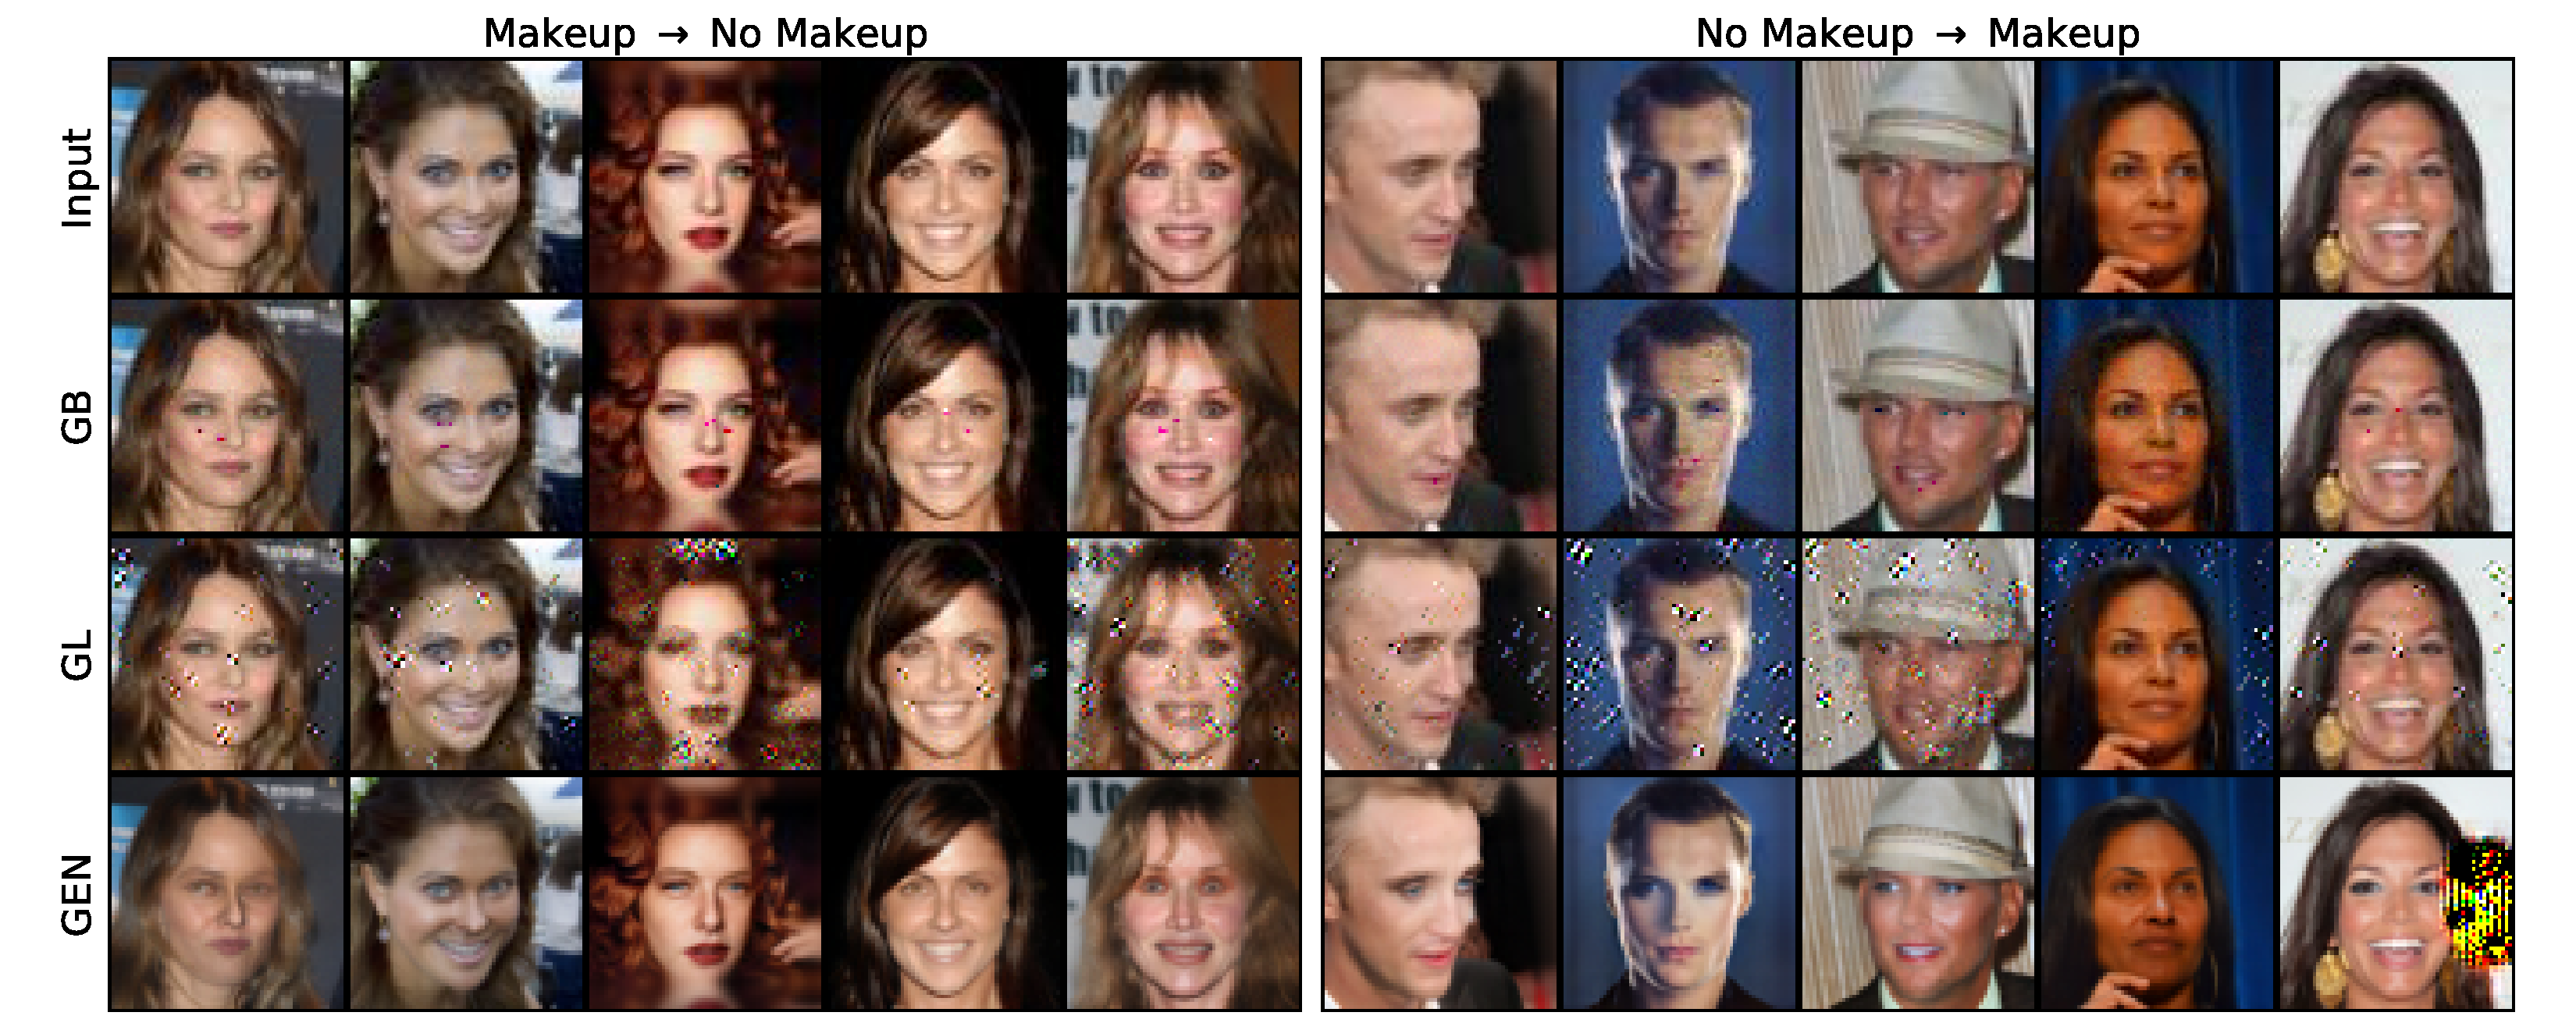
\includegraphics[trim={0, 10, 0, 0}, clip, width=\textwidth]{graphics/celeba.pdf} 
    \caption{First row is input images. Second to fourth row is counterfactual examples on the makeup vs. no makeup label, generated by \cite{Wachter2017} (GB), \cite{VanLooveren2019} (GL), and ECINN (GEN), respectively. The first five columns converts people with makeup to people without, and vica versa for the last five columns. The figure is a direct copy of an old version of a figure from \paperref{pap:evaluation}.}
    \label{fig:iterative-counterfactuals-copied}
\end{figure}
\begin{figure}[b]
    \centering
    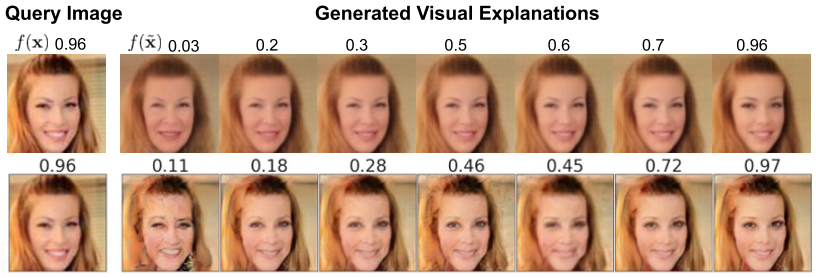
\includegraphics[width=\linewidth]{graphics/generative.png}
    \caption{Counterfactuals explanations on the old vs. young label generated by \cite{Rodriguez2021} (first row) and \cite{Singla2019} (second row). The figure is a composition of figures copied directly from the two papers.} 
    \label{fig:generative-counterfactuals-copied}
\end{figure}

Analytically choosing the counterfactual is the last property that we highlight here.
The benefit of analytical solutions to the counterfactual problem is a tight relationship between the theoretical properties of the classifier and the associated counterfactual examples.
% \todo{This needs a much better motivation. Could phrase it like theoretically grounded approaches. However, one could argue that other methods are also theoretically grounded?} 
It becomes possible to prove guarantees on the counterfactual examples, which may be favorable in some situations. 
Of the presented methods, only ECINN has an analytical solution, where counterfactual examples situated exactly on the decision boundary between two classes is possible to produce.
Of course, the analytical approach of ECINN comes at a cost.
% The method is based on a particular type of neural networks, which can be inverted and for which the Jacobian determinant computations are tractable.
% Only few network architectures have those properties.
% However, as demonstrated in \cite{iresnet}, the widely used and high performing ResNet classifier \cite{resnet} can be constrained to have an inverse by normalizing the weights of the network by their spectral norm.
% A caveat is, however, that sampling becomes less efficient for such networks. 
% Consequently, ECINN can also be applied to the powerful ResNet architecture, to potentially obtain both high performance on accuracy and high quality counterfactuals. 
% 
% There is an inherent drawback of ECINN, which should be mentioned.
Our method only applies to conditional Normalizing Flows, where the other methods mentioned apply to any classification model $f$ which supports gradient computations.
Recent work on Normalizing Flows~\cite{iresnet, ffjord, expl-inn} does, however, indicate that conditional Normalizing Flows can be extended to popular model architectures like ResNets~\cite{resnet} under mild model constraints. 
For example, \cite{iresnet} demonstrate that if the weights of a ResNet are normalized by their spectral norm, their inverse can be computed and Jacobian determinant estimated at the cost of a less efficient sampling process.
Applying ECINN to such model architecture would most likely result in a less efficient generation process for the counterfactual examples, but achieve better classification accuracies.
\citet{expl-inn} further demonstrate how a modification of a ResNet architecture to make it invertible yields similar or slightly worse accuracies on ImageNet~\cite{imagenet} as compared to the original ResNet, but retains the efficient sampling procedure and well-structured latent space.
As such, we are optimistic that ECINN can successfully be applied to more powerful and popular architectures.
    
With ECINN, we have introduced a promising new direction of research within the field of counterfactual examples. 
ECINN utilizes the benefits of generative models while having an analytical solution, in contrast to related work, which needs additional optimizations to either find counterfactual examples or pretrain external generative models.
ECINN produces high-quality counterfactual examples that are visually on par with other methods based on generative models, and better than counterfactuals generated by iterative methods.
In the next chapter, we change the perspective from particular methods for producing counterfactuals to how to quantitatively evaluate counterfactual examples. 


% % % % % % % % % % %  % % % % %  % % % % %  % % % % %  % % % % %  % % % % %  % % % % % 
% EVALUATING COUNTERFACTUALS
% % % % % % % % % % %  % % % % %  % % % % %  % % % % %  % % % % %  % % % % %  % % % % % 
\chapter{Evaluating Counterfactual Examples}\label{chap:evaluation}
% +++  1 page of introduction to the problem
Central for the development of any field of research are practices for evaluating methods proposed within the field.
For counterfactual examples, both ``objective'' and ``subjective'' methods have been proposed to evaluate different aspects of the generated examples~\cite{Stepin2021}.
Objective methods are automatic corpus-based metrics, including, \eg, accuracy and number of features changed.
In contrast, subjective methods are based on human judgment like, \eg, relevance or interpretability, as judged by humans.
As indicated by the name, objective metrics are beneficial because they can be applied objectively across different publications in order to quantify performance.
As we demonstrate in \paperref{pap:evaluation}, objective metrics used for image counterfactuals sometimes fail to distinguish the good from the bad examples.
% The particular issue is perhaps also one of the reasons why subjective metrics have been proposed.
This chapter focus on objective metrics for image counterfactuals. 
We first give a high-level overview of desired properties of image counterfactuals before describing existing metrics that have been proposed to quantify such properties in Section \ref{sec:existing-metrics}.
Afterward, Section \ref{sec:evaluation-paper} describes how \paperref{pap:evaluation} contributes with a better understanding of what properties existing metrics do and do not capture, as well as two new metrics that mitigate drawbacks of existing metrics.
The chapter is concluded with a discussion in Section \ref{sec:eval-discussion}.

\paragraph{Desired properties.}
As formulated in \citet{Wachter2017}, counterfactual methods should find \emph{minimal} and \emph{necessary} changes to the input such that the predicted class changes.
% Also diversity among multiple counterfactuals for the same input is mentioned as being valuable.
For images, \citet{Mothilal2020} further describe validity, sparsity, proximity, and diversity as properties that good counterfactual examples should possess.
Necessary changes are closely related to validity, while sparsity and proximity are concerned with minimal changes. 
Below, we briefly describe the four properties from \cite{Mothilal2020} that are afterward used to categorize existing metrics.

\begin{description} 
    \item[Validity] is closely tied to necessary changes by accounting for whether the predicted class actually changes. 
    Quantitatively, validity is the proportion of counterfactual examples that yield a different predicted outcome than the original input.
    A high validity is essential for counterfactual methods to be useful in practice.
    Validity is directly quantifiable and poses no challenge to evaluate.
    
    \item[Sparsity] relates to how many features are changed from the input to the generated counterfactual.
    As argued in, \eg, \cite{Wachter2017} and \cite{Grath2018}, the sparsity of an explanation constitutes a proxy for how interpretable a counterfactual example is, \ie, the more sparse the counterfactual change is, the more interpretable the counterfactual is. 
    Depending on the domain, sparsity can be hard to quantify because sparse changes can relate to changing a few semantic features rather than, \eg, a few pixel values.
    
    \item[Proximity] is closely related to sparsity and minimal changes by considering how close generated counterfactuals are to their associated input.
    According to \citet{Mothilal2020}, a counterfactual close to the input can be most useful to the users.
    The difficulty of quantifying proximity also depends on the domain, as we will discuss in this chapter. 
    
    \item[Diversity] revolves around producing a diverse set of counterfactuals for each input.
    When a user is presented with multiple diverse counterfactuals, more information about the classifier under consideration will consequently be conveyed and increase the likelihood of finding valuable explanations~\cite{Rodriguez2021}.
    In \paperref{pap:evaluation}, we do not consider diversity, as we have not identified any established metric (used by more than one publication) for quantitatively comparing diversity.
    We will, however, cover aspects of quantifying diversity below.
\end{description}

In addition to the four mentioned properties, many publications, including our \paperref{pap:ecinn}, further revolve around realistic counterfactuals~\cite{Singla2019, flowcounterfactuals, Rodriguez2021, VanLooveren2019}. % TODO connectedness papers
Realistic counterfactuals can be interpreted as samples that are likely to stem from the same distribution as the training data. 
Therefore, quantifying how realistic counterfactual examples are has mostly been done by various density estimates or proxies thereof.
In the following, we will also discuss such quantities. 

% \section{Quantifying performance of Counterfactual Examples}  
\section{Existing Quantitative Metrics}\label{sec:existing-metrics}
% +++ 3 pages of related work. 
% Describe the metrics for tabular data and describe how they do not apply to images, either because of computational complexity,
% characteristics of images, or other issues.
% Then describe what has been done on images. 

This section describes quantitative metrics that have been used to evaluate counterfactual methods proposed within the image domain.
Although not all metrics fit perfectly into the properties listed above, we describe them in the context of such properties to give an overview of which properties that can be evaluated by existing metrics.

\paragraph{Validity.}
As mentioned, the proportion of generated counterfactuals that successfully change the predicted class, \ie, the validity or target-class validity as denoted in \paperref{pap:evaluation}, is straight forward to quantify.
Let $f$ be the classifier under consideration and $c: \mathcal{X} \rightarrow \mathcal{X}$ be the counterfactual method that produces a counterfactual example for inputs $x\in \mathcal{X}$ from some domain $\mathcal{X}$, then the target-class validity ($\operatorname{TCV}$) is defined as
\begin{equation}\label{eq:tcv}
    \operatorname{TCV} = \frac{1}{|X|} \sum_{x \in X} \mathbb{1}_{[ f(x) \neq f( c(x) )]}, 
\end{equation}
where $\mathbb{1}_{[\cdot]}$ is the indicator function and $X \subset \mathcal{X}$ is the dataset being explained.
A larger $\operatorname{TCV}$ is better, as more counterfactuals successfully change the predicted class.

\paragraph{Sparsity.}
Depending on the domain, sparsity can be hard to quantify.
For tabular data with relatively few features or for text, sparsity can simply be ``counted''~\cite{Kang2020, Laugel2018} to give an idea of the complexity of an explanation. 
% If a sentence is altered to form a counterfactual sentence, then it can be of value to ``count'' how many words were changed to quantify how sparse the counterfactual example is~\cite{}.
In the image domain, it is harder to quantify sparsity in a meaningful way.
In fact, we know of no publications within the image domain that report sparsity.
As an example of why sparsity can be less useful, \cite{one-pixel-attack} demonstrates how changing just one pixel in an image can be enough to change the prediction of a neural network.
Such a change is sparse but is most likely of little or no use to the end-user.
A more meaningful way of measuring sparsity in the image domain would be to quantify how many semantic features change between the input and the counterfactual.
However, we know of no work that quantify semantic sparsity with the purpose of evaluating counterfactual examples.
% However, computing, \eg, the $L1$ distance between the input and the counterfactual to quantify sparse changes is of less use~\cite{Kang2020}. 
% Again, adversarial attacks can obtain a low $L1$ distance without conveying any useful information to the user.
Although sparsity is not reported within the image domain, \eg, the $L1$ metric which is closely related to sparsity is frequently used as a part of optimization losses when generating visual counterfactual examples~\cite{VanLooveren2019, Dhurandhar2018, Wachter2017, Singla2019}. 

\paragraph{Proximity.}
For proximity, the ``distance'' from an input to a generated counterfactual needs to be quantified.
\citet{Mothilal2020} measure proximity by the average $L1$ distance normalized by the median absolute deviation of each feature (defined in Equation \eqref{eq:MAD}) from the input to the counterfactual. 
Notably, this relates closely to sparsity, which makes the mathematical distinction between the two unclear.
\cite{Mothilal2020} highlights both sparsity and proximity as being important, but quantifies only sparsity.

As was the case for sparsity, quantifying proximity may seem trivial, but using, \eg, the $L2$ norm to measure proximity often falls short.
Take the image domain as an example.
In Figure \ref{fig:l2-example}, an image of a seven (left) is altered in two ways. 
In the center image, the digit is rotated seven degrees, and in the right image, the tip of the top line has been cut off.
Perceptually, the center image is arguably more proximal to the input than the right image.
However, according to the $L2$ distance, the right image is closer.
As such, using simple norms to quantify proximity can be inadequate.
We hypothesize that similar observations can be done for other high-dimensional domains.

\begin{figure}
    \centering
    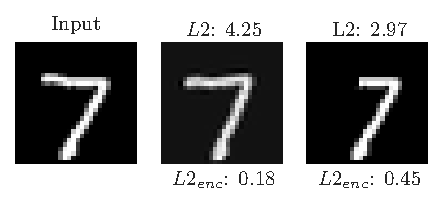
\includegraphics[trim={0, 17, 0, 0}, clip]{graphics/l2-example.pdf}
    \caption{L2 distance between an input and two modifications. The center image is rotated seven degrees and the right image has tip removed.}
    \label{fig:l2-example}
\end{figure}

Both for image classification and many other high-dimensional tasks, it is generally believed that the data lies on a manifold of much lower dimension than the data dimension, see, \eg, \cite[Sec. 3.11.3]{Goodfellow-et-al-2016}.
Consequently, metrics like the FID try to approximate such manifolds to quantify similarity on the manifold \cite{fid}.
In the context of counterfactual examples, there exist only one work that quantifies proximity in a latent space.
Particularly, \citet{Rodriguez2021} use an oracle classifier trained on a related dataset (VGGFace2~\cite{vgg2faces}) to that being explained (CelebA~\cite{celeba}) and reported the cosine distances between embedded images.
% To demonstrate the effectiveness of such an approach, we trained a small VAE to reconstruct digits.\footnote{The VAE had three dense ReLU activated layers of 400 hidden dimensions in the encoder and decoder. It was trained for 30 epochs on MNIST with the ADAM optimizer~\cite{adam}. Model architecture and training code is available at \url{https://github.com/singhgautam/vae-pytorch}}
% As indicated in Figure \fref{fig:l2-example}, even such a simple model with no advanced engineering applied yields more meaningful $L2$ norms in its embedding space.
% As the metric was not found to be used by other papers, we have not included it in \paperref{pap:evaluation}, but we highlight it here as a promising direction for quantifying proximity.

It should also be mentioned that \cite{Rodriguez2021} presents FID as a way of quantifying proximity.
We do, however, argue that the FID does not quantify proximity as such.
The reason is that the FID is a population-based metric, \ie, it yields one score for counterfactuals generated across many inputs.
In turn, shuffling counterfactuals, such that they become associated with different (non-proximal) inputs, will yield the same FID score.
As such, a counterfactual method may get a low (good) FID by producing realistic counterfactuals that are \emph{not} proximal to their associated inputs.
Therefore, we cover FID in the ``Realistic counterfactual examples'' paragraph below. 

Finally, \citet{Singla2019} evaluate how sensitive different predicted class labels are to changes made by the counterfactual method. 
That is, they quantify how often other class labels than the target class are predicted to change when counterfactual examples are generated. 
Although not presented as such in the paper, quantifying such changes relates to ``semantic proximity'' by measuring how different semantic features change with the counterfactual examples. 

\paragraph{Diversity.}
As \citet{Mothilal2020} and \citet{Wachter2017} describe, diversity is important to convey more comprehensive information about the classifier being explained.
Despite not mentioned explicitly, diversity is injected into multiple methods for generating counterfactual examples including our \paperref{pap:ecinn}~\cite{Joshi2018, Singla2019, Rodriguez2021}. 
However, there does not seem to exist any established metrics for quantifying diversity among counterfactual examples.

\cite{Mothilal2020} quantifies diversity as the average distance among pairs of counterfactuals generated for the same input. 
As for sparsity, the distance used is the $L1$ distance normalized by the median average deviation.
As argued above, metrics based on the $L1$ norm make less sense for, \eg, images.
We are also not aware of any other work that reports this metric.

It should be mentioned that for text, the self-BLEU score~\cite{self-bleu} has also been proposed to quantify diversity between counterfactual examples~\cite{Wu2021}.
However, the score does not extend naturally to the image domain and is not covered further here.

\paragraph{Realistic counterfactual examples.} 
Another property that counterfactual examples should possess is that they should be realistic.
For images, realistic counterfactual examples would ideally be images that end-users cannot tell are synthetic. 
Such property can be hard to quantify.
% Metrics typically use likelihood as a proxy for how realistic data is. 
% That is, metrics approximate the likelihood of the counterfactuals examples to stem from the distribution that generated the training data. 
%
When the true causal structural model that generated the data is known (typically only in synthetic/toy examples), it is possible to exactly quantify the likelihood of counterfactual examples under the causal model~\cite{Mahajan2019}. 
The exact likelihood is a good indication of how realistic the counterfactual examples are. 
However, in a deep learning setting described with Problem Statement \ref{def:dl-counterfactual}, exact likelihood computations under the true data-generating distribution is not possible. 
Instead, it is common to approximate the distribution of the data to quantify the closeness of the data to that distribution~\cite{VanLooveren2019, flowcounterfactuals, Singla2019, Rodriguez2021}.

In the image domain, examples of metrics that revolve around realistic changes are the two interpretability metrics $\operatorname{IM1}$ and $\operatorname{IM2}$ presented by \citet{VanLooveren2019} and the FID used in \cite{Singla2019, Rodriguez2021}. 
As discussed in the previous chapter, \citet{flowcounterfactuals} further prove that their generated counterfactual examples will approximately stay on the data manifold of the training data, which must be expected to generate more realistic counterfactual examples.

Although presented as an interpretability metric in \cite{VanLooveren2019}, the authors describe how the $\operatorname{IM1}$ score approximates how close the counterfactual examples are to the data manifold by comparing how well auto-encoders, trained on different subsets of the training data, reconstruct the counterfactuals. 
The metric is defined as 
\begin{equation} 
    \label{eq:IM1} 
  \operatorname{IM1}\left( x, p, q \right) = 
        \frac{
            \left\|c-\mathrm{AE}_{q}(c(x))\right\|_{2}^{2}}
        {
            \left\|c-\mathrm{AE}_{p}(c(x))\right\|_{2}^{2}+\epsilon
        },
\end{equation}
where $p$ and $q$ are the input and target classes, respectively, and $AE_i$ is an auto-encoder trained on training data only from class $i$. 
Intuitively, if $c(x)$ successfully transforms $x$ into class $q$, $AE_q$ should be able to reconstruct the counterfactual $c(x)$ with a lower reconstruction error than $AE_p$, thus yielding an $\operatorname{IM1}$ score less than one.
The score has been reported in multiple papers~\cite{VanLooveren2019, Mahajan2019, Schut2021}. 

\citet{VanLooveren2019} also propose the similar $\operatorname{IM2}$ score to quantify how interpretable counterfactual examples are. 
The score uses an auto-encoder $AE$ that is trained on the full training set: 
\begin{equation}\label{eq:IM2}
\operatorname{IM2}\left(x, q\right)=\frac{\left\|\mathrm{AE}_{q}\left(c(x)\right)-\mathrm{AE}\left(c(x)\right)\right\|_{2}^{2}}{\left\|c(x)\right\|_{1}+\epsilon}.
\end{equation}
According to the authors, if the score is low, then the distribution of the target class $q$ describes $c(x)$ as well as the distribution of all classes.
In turn, a low score should represent a more interpretable counterfactual.
%
%According to the authors, the intuition is that if the score is low, then the distribution of the target class $q$ describes $c$ as well as the distribution of all classes, which should represent a more interpretable counterfactual.
It is, however, debatable whether the $\operatorname{IM2}$ score quantifies interpretability.
For example, \citet{Schut2021} find that the score fails to distinguish in- and out-of-distribution samples, which refrain them from reporting the score.
In any case, the $\operatorname{IM2}$ score relates to realistic changes by having auto-encoders reconstruct the counterfactual examples.
If the reconstruction errors are high, this hints that the given counterfactual does not resemble the training data.
% In turn, the score is not reported in \cite{Schut2021}. 

Another way to quantify how realistic counterfactual examples are is to use the FID.
As discussed in Chapter \ref{chap:nns}, FID is a well-established metric within the field of generative models.
As counterfactual methods also generate synthetic samples, it is reasonable to apply the metric in this field as well.
Despite denoting it data consistency, \cite{Singla2019} utilize the FID to evaluate how realistic counterfactual examples are, \ie, how close the counterfactuals are to the data manifold.
As mentioned, \citet{Rodriguez2021} also apply the FID to evaluate visual counterfactual examples. 
Although it is denoted proximity in \cite{Rodriguez2021}, we argue that the metric is more a measure of how realistic counterfactual examples look due to the population-wide nature of the metric.

Finally, various forms of ``connectedness'' have also been proposed to capture whether counterfactuals stay in the vicinity of the training data~\cite{Laugel2019, Pawelczyk2020, Poyiadzi2020}, arguably to quantify whether they are realistic. 
A counterfactual and a real data point is said to be $\varepsilon$-connected, if a chain of points connecting the two exists. 
All links in the chain need to be within an $\varepsilon$-distance to each other and the same predicted class~\cite{Laugel2019}.
% Overall connectedness can then be computed as the percentage of counterfactuals that are connected to at least one point from the training data.
If a counterfactual example is $\varepsilon$-connected to a known point, then the counterfactual is intuitively ``justified'' by approximately being in a high-density region of the particular target class. 
However, it can be costly to compute such connectedness due to the high dimensionality of many domains.%\footnote{Although for ECINN, we can actually find such chain by searching for embeddings on a straight line between the counterfactual and any sample predicted to be of the same class in the latent space of the INN, as the latent decision boundaries are also linear.}

In \paperref{pap:evaluation}, we discuss the $\operatorname{IM1}$, $\operatorname{IM2}$, and FID metrics further to reveal both pros and cons of the metrics.
The next section highlights our contributions in the domain of evaluating visual counterfactual examples. 

\section[On Quantitative Evaluations of Counterfactuals]{On Quantitative Evaluations of Counterfactuals\contribution{pap:evaluation}}\label{sec:evaluation-paper}
% +++ 3 pages on our contributions.

% Introduction: 
% - Above, we have described counterfactual properties through five points. This is to give the reader an idea of how unestablished the field of objevtively quantifying the quality of counterfactuals is. 
% - We believe that the place to start is with lack of konwledge about what established metrics actually quantify, which is what pap:evaluation revolves around.
Above, we have described existing metrics in terms of the five properties broadly agreed to be important for visual counterfactual examples.
The intention is to give insights into the lack of proper metrics within the field. 
Specifically, we find that sparsity, proximity, and diversity are left largely unquantified. 
Due to the lack of well-established metrics, \paperref{pap:evaluation} generalize sparsity and proximity to minimal changes and only briefly mentions diversity. 
However, it should be stressed that for future work, it is important to quantify such properties.
% In our paper, we focus on understanding the behavior of existing metrics, which make us generalize the desired properties to minimal and realistic changes for simplicity. 

It may be clear to the reader that quantitatively evaluating counterfactual examples is not a solved problem.
Especially for visual counterfactual examples, quantitative metrics are limited, and knowledge about what properties metrics do capture and do not capture is even more scarce.
We believe that a thorough understanding of the behavior of existing metrics is the best first step before designing new metrics to establish a best practice for evaluating visual counterfactual examples.
This insight is what motivates our work in \paperref{pap:evaluation}, which, through analysis and experimental evaluations, takes a step towards improving the quantitative evaluations of visual counterfactual examples.

% Whats in the paper.
\paragraph{Contributions.}
The paper consists of three main contributions.
An analysis, experimental evaluations, and two new metrics for evaluating counterfactual methods.
We analyze established metrics in the context of visual counterfactual examples, and we do multiple experiments on datasets of increasing complexity. 
% Throuobserve which properties metrics capture and what properties they do not capture.
Through our analysis and experiments, we demonstrate what properties metrics do and do not capture. 
For example, we find that tiny adversarial-like changes, sometimes produced by, \eg, the method from \cite{Wachter2017}, get undesirable good scores according to multiple metrics.
To mitigate this issue, we introduce two new metrics, which rely on ``oracle'' classifiers to avoid promoting such adversarial-like counterfactuals.
In the following, we summarize our findings before presenting the two new metrics that we propose.

% Theoretical
% - Discussion of how each metrics quantifies some properties, but cannot stand alone,  because they can be fooled.
% - Metrics should be reported together to form a more comprehensive profile of the evaluated method.
% - Sharing models and data normalization is important!
% - No metric for quantifying whether label-independent features change => We introduce LVS (and oracle score)
\paragraph{Analytical findings.}
Through our analysis of existing metrics that have been reported in at least two publications, we generally find that all metrics capture properties at the cost of leaving other properties unattended.
The consequence is that they become vulnerable when considered in isolation.
Take FID as an example.
As we described, shuffling the relationships between inputs and counterfactuals will yield the same FID.
In turn, we conclude that FID should be considered along with other metrics, which do not have this issue.
Similarly, $\operatorname{TCV}$ captures how effective a counterfactual method is in changing the predicted class. 
% As discussed in \paperref{pap:evaluation}, the metric provide valuable insights into how effectively methods produce counterfactuals.
On the other hand, the metric does \emph{not} convey any information on the image quality.
Adversarial attacks may, \eg, get a high (good) $\operatorname{TCV}$ but convey little or no information to the end-user, as such attacks are typically not interpretable.
Consequently, $\operatorname{TCV}$ also needs to be considered along with other metrics that do not have this drawback.
Overall, we find that no metric expresses all desirable properties. In turn, they should be used in combination.

In \paperref{pap:evaluation}, we also point out that reporting the normalization used for evaluating counterfactuals is crucial for comparing methods across publications.
In the existing literature, we observe that the $\operatorname{IM1}$ and $\operatorname{IM2}$ metrics are reported for two different ranges of normalization in \cite{Mahajan2019} and \cite{VanLooveren2019}, which leads to incomparable results.
This issue is apparent for metrics that use, \eg, the $L2$ distance, which is affected by normalization.
For reproducibility and to enable comparisons across publications, we also stress that metrics like the $\operatorname{IM1}$ score and the FID that are based on pretrained machine learning models make it crucial to also share the exact models used.
With \paperref{pap:evaluation}, we also publish code for evaluating visual counterfactual examples.\footnote{\url{https://github.com/fhvilshoj/EvaluatingCounterfactuals}}
With the code, normalization and model parameters for the ``evaluation models'' are handled automatically.
In turn, if future publications use our code, comparison across publications becomes possible.

% Practical
% - Adversarial attacks are annawying.
% - We tie FakeMNIST together with the LVS and find that all considered metrics yield meaningful results in this controlled environment. 
% - On MNIST, which is an often used (within counterfactual experiments) and easy dataset, we find that some metrics fail when compared to human interpretation. 
% - With the more complex Celeba-HQ dataset, we ...
\paragraph{Experimental findings.}
With our experiments, we confirm multiple of our analytical observations.
First, we confirm that normalization does matter.
We demonstrate that comparing the $\operatorname{IM2}$ score across two different normalizations potentially yield wrong conclusions if one counterfactual method with one normalization is compared to method with another normalization. 
Second, we demonstrate that both simple norms of differences between inputs and counterfactuals, FID, and the $\operatorname{IM1}$ and $\operatorname{IM2}$ will wrongly give good scores to counterfactuals that are less meaningful to the user.
For example, we examine extreme cases where counterfactuals that consist of tiny adversarial-like changes and images without any information (all black images) yield better scores than realistically looking counterfactuals according to the $\operatorname{IM1}$ and $\operatorname{IM2}$, respectively.
Similarly, for the MNIST dataset, FID yields a lower (better) score for adversarial-like changes than more realistically looking counterfactual examples.

Comparing our experiments across an increasing data complexity reveals that the $\operatorname{IM1}$ and the $\operatorname{IM2}$ scores across different counterfactual methods seem to approach identical values.
That is, when complexity increases, the difference between methods decreases.
In turn, such metrics are arguably most valuable for less complex data.

\paragraph{New metrics.}
From our analysis and experiments, we found that the evaluated metrics for quantifying realistic changes can be fooled by adversarial-like examples.
Consequently, we introduce two new metrics that help quantify realistic changes without giving good scores to such small changes.
First, we introduce the oracle score, which is similar in construction to the $\operatorname{TCV}$, but uses a surrogate ``oracle'' for the evaluation.
The oracle score is the proportion of counterfactuals where the classifier $f$ agrees with the oracle $o$ on the counterfactual class: 
\begin{equation}\label{eq:oracle}
    \operatorname{Oracle} = \frac{1}{|X|}\sum_{x\in X} \mathbb{1}_{[ f(c(x)) = o(c(x)) ]}.
\end{equation}
The score is based on the assumption that adversarial attacks are highly model-specific~\cite{Liu2017}.
Under this assumption, the Oracle score should be high if changes are realistic such that both $f$ and $o$ capture the change in class, while adversarial attacks should only affect $f$.
In our experiments, the assumption is verified by the score consistently giving better (higher) scores to realistically looking counterfactuals.

For datasets where inputs have multiple class labels, we further introduce the Label Variation Score (LVS), which also captures aspects of realistic changes without giving good scores to tiny adversarial-like changes.
At a high level, LVS is based on the assumption that for an image of a face with makeup, when a face without makeup is generated as a counterfactual example, other semantic features like gender and hair color should not change.
To capture this, LVS uses multiple oracles trained to recognize different class labels like, \eg, hair color and gender to quantify how much these label-independent features change. 
LVS computes average Jensen-Shannon divergences $D_{js}$ between inputs and associated counterfactuals to quantify such changes.
For oracles $o_l$, trained on $L$ distinct class labels $l\in \{1,...,L\}$, which outputs a discrete probability distribution over the labels, the LVS is defined as 
\begin{equation}\label{eq:lvs}
   \operatorname{LVS}_l = \frac{1}{|X|} \sum_{x \in X} D_{js}\left[ o_l(x) || o_l(c(x))\right].
\end{equation}
In turn, LVS provides a score for each class label in the dataset.
In general, good scores should be such that the target class label gets a high score, while other labels get low scores.
There may also be situations where different class labels complement each other. 
For example, makeup is arguably associated (correlated) with lipstick, which may thus also attain a higher score.
We leave it to domain experts to judge which class labels may meaningfully get higher scores along with the target label of the counterfactual example. 
We find experimentally that the LVS yields scores that align with human interpretation, and tiny adversarial-like changes consistently get worse scores than more realistically looking counterfactuals.

\section{Discussion}\label{sec:eval-discussion}
% +++ 1 page of discussion 
% How does our work relate to the field?
% What are the consequences of our contribution?
% - We believe that our work constitutes a step in the right direction for establishing best practice metrics for objectively evaluating counterfactual examples.
% - More complex datasets. I am not aware of any metrhod that surpass Celeba? Unless it is by translating counterfactual exmples into heatmaps, using gaussian blur, boundingboxes and what not \cite{cf-heatmap-imagenet}
% - Inference time is of course also important, but poses no challenge in terms of quantification and does not seem to be suceptible to being fooled.
% - LVS only works for datasets with multiple class labels.
As the amount research on counterfactual examples has increased rapidly recently~\cite{Stepin2021}, we find it crucial for the field to have proper benchmarks against which counterfactuals can be compared.
At the time of writing, we only know of one very recent work, which presents a framework with a suite of metrics for evaluating counterfactual examples on low-dimensional data~\cite{clara}. 
The framework comprises metrics like $L1$ distance, $\operatorname{TCV}$, and connectedness, which we argued are of little or no use in, \eg, the image domain.
As such, we find the timing of our paper to be just right. 
With \paperref{pap:evaluation}, we have taken an essential step towards establishing a standard suite of metrics for evaluating visual counterfactual examples, for which there exists a solid understanding of which properties each metric does and does not capture.
Our work constitutes a steppingstone towards designing new metrics that successfully capture properties like sparsity, proximity, and diversity.
Such metrics are crucial for improving further progress within the field of counterfactual examples.

Perhaps the most pronounced concern that the reader may get from reading \paperref{pap:evaluation} is the complexity of the datasets used in the experiments. 
Today, visual deep learning models can be applied to datasets with huge complexities~\cite{biggan, vit}, much larger than those used in our experiments.
In turn, we do not know whether our results extend to such complexities.
Except \cite{Elliott_2021_CVPR} that computes heatmaps on ImageNet~\cite{imagenet} from discrepancies between inputs and counterfactuals, we know of no counterfactual method for which experiments extend beyond the complexity of the CelebA dataset~\cite{celeba}.
Our experiments extend to the $64\times 64$ pixel downscaled version of the CelebA-HQ dataset~\cite{celeba-hq}. 
As such, we are close to, but not at the limit of, the data complexity of related work.\footnote{We used CelebA-HQ in a down scaled $64\times 64$ pixel version, due to limited resources.}
% it was not possible for us to extend our experiments to such datasets within a reasonable time budget. 
% It should be mentioned that \citet{Elliott_2021_CVPR} does scale experiments beyond CelebA. 
% However, they use counterfactual examples to generate heatmaps from the discrepancies between inputs and counterfactuals on the ImageNet dataset~\cite{imagenet}. 
% We hypothesize that the authors transform counterfactuals into heatmaps because the counterfactuals do not look realistic as-is.

Finally, a conclusive strategy for evaluating visual counterfactual examples may also seem to be missing in \paperref{pap:evaluation}. 
However, metrics are still missing in terms of giving a complete evaluation of the five properties described above.
As such, presenting a conclusive strategy could potentially harm further development by ignoring the missing aspects. 
In turn, we refrain from giving such a strategy. 

% Future work:
% NB this is very important to mention somewhere, as the reader might get wrong expectations.
% - There is still a long way to go in terms of quantifying, e.g., sparsity, and proximity.
% - It is surprising that no one evaluated proximity, sparsity, diversity, and likelihood in the latentspace of some powerful neural network. This constitutes a very exiting new direction of research.
%
    
\chapter{Conclusion} 
Having summarized the four included papers during the previous three chapters, we conclude Part \ref{part:overview} of this thesis in this chapter.
In Section \ref{sec:conclusion-discussion}, our work is discussed in terms of the main hypothesis and the associated research questions. 
Section \ref{sec:conclusion-conclusion} concludes our contributions and Section \ref{sec:conclusion-future-work}. 
presents promising future work. 

\section{Discussion}\label{sec:conclusion-discussion}
% 1.5 page on how presented work relate to our research questions and the main hypothesis in general.
Recall that the main hypothesis of this thesis is that crossing generative models with explainability can yield state-of-the-art explainability techniques. 
We have shed light on this hypothesis through three different research questions.

In Chapter \ref{chap:nns}, we have presented two answers for the first research question; how can we improve training efficiency?
As it should be clear that both FastH and FastFID speed up computations used for training neural networks and, as a consequence, allow scaling data or model sizes within a limited computational budget, we seize the opportunity to illustrate how both algorithms could improve explanations.
Taking ECINN as an example, we could, as described in Section \ref{sec:fasth-applications}, employ the FastH algorithm to compute determinants and inverses of certain layers of Normalizing Flows faster.
Faster computations mean larger scale, which typically yields higher generative performances.
With higher generative performance, we would expect ECINN to produce better counterfactual examples. 
With the FastFID algorithm, we could imagine adding the FID loss when training the conditional Normalizing Flow, which, in the setup proposed with ECINN, is used for both classification and generation of counterfactual examples.
Adding the FID loss could potentially yield counterfactual examples of higher visual quality.
For the interested reader, \paperref{pap:fastfid} present an experiment where the FID loss is added to a regular Normalizing Flow.
Applying the FID loss to Normalizing Flows does, however, result in visual artifacts.
It constitutes a direction of future work to derive a proper training mechanism for Normalizing Flows with an additional FID loss. 

In Chapter \ref{chap:ecinn-main}, we presented ECINN, which addresses our second research question; how can generative models be used to explain neural networks?
ECINN utilizes the generative capacities of conditional Normalizing Flows to generate counterfactual examples. 
While related methods that use generative models typically use the generative models as external image generators that produce more realistically looking counterfactuals, ECINN directly utilizes the generative capabilities of the classifier at hand. %, which can both be used for classification and conditional sampling.
The method represents a new direction of research where generative models are \emph{not} used as an external generators but internal parts of the classification networks.
We hypothesize that such a close relationship between the classifier and the generator can lead to counterfactuals that closely reflect the actual behavior of the classifiers. 

In Chapter \ref{chap:evaluation}, we considered the third research question; how can we best evaluate explanations?
We provide insights into what properties existing metrics for evaluating visual counterfactual examples capture and further introduce two new metrics.  
The discussion in Chapter \ref{chap:evaluation} further establishes that the suite of metrics for evaluating visual counterfactual examples is still not complete.
We believe that the contributions of \paperref{pap:evaluation} constitute an important steppingstone towards better evaluation metrics for visual counterfactual methods.

Despite not being the main intention of \paperref{pap:evaluation}, the paper presents experiments which indicate that ECINN, as a representative of methods that are based on generative models, quantitatively produce better counterfactual examples than representatives of iterative methods. 
As we have argued that the set of evaluation metrics is still not complete and because we did not evaluate all counterfactual methods, we cannot determine which counterfactual method holds the state-of-the-art.
Even though the results presented in both \paperref{pap:ecinn} and \paperref{pap:evaluation} indicates that counterfactuals based on generative models are of higher quality than those that do not use generative models.
In turn, we fail to reject our main hypothesis that explanations based on generative models can produce state-of-the-art results.
As such, we continue to believe that there is great potential within this line of research.

% To conclude on our main hypothesis, we find in \paperref{pap:evaluation} that methods based on generative models produce bettt
% However, from the metrics which currently exist and from qualitative inspections, we found that ECINN outperforms methods that are not based on generative models.
% Furthermore, ECINN seems to qualitatively perform roughly on par with other approaches for generating counterfactual examples, such as those from \citet{Singla2019} and \citet{Rodriguez2021}, that are based on generative models. 
% ECINN does, however, have the additional property that it is based on an analytical solution instead of an optimization problem. 
% It is inconclusive which of ECINN and the other methods based on generative models holds the state-of-the-art within visual counterfactual examples.


\section{Conclusion}\label{sec:conclusion-conclusion}
% 0.75 page concluding our contributions.
In this thesis, we have focused on combining generative models and the field of explainability.
The research has been driven by the assumption that such a combination can produce state-of-the-art methods for explainability. 
We have introduced two published papers and two manuscripts, each of them contributing directly or indirectly to the field of explainability by the connection to our three research questions. 
Below, we outline the main contributions of each paper.

With \paperref{pap:svd}, which was published as a Spotlight paper at NeurIPS, we introduced FastH, a novel GPU-friendly algorithm for evaluating products of Householder matrices fast.
The algorithm enjoys the fast asymptotic time complexity of a previously proposed sequential algorithm but with less sequential work.
The algorithm is up to $27\times$ faster than the sequential algorithm.
With FastH, it is possible to parametrize weights of neural networks in their SVD efficiently.
Such parametrization allows efficient computations of, \eg, the matrix determinant, the matrix inverse, and spectral normalization, all computations that are used in generative modelling. 
As FastH can be plugged directly into the conditional Normalizing Flows used by our method ECINN, it can potentially improve the explanations of ECINN further downstream.

With the manuscript in \paperref{pap:fastfid}, we introduced FastFID, an algorithm that allows computing the FID efficiently for small mini-batches.
When the mini-batches are sufficiently small, FastFID can be three orders of magnitude faster than the original implementation of FID. 
With this significant speed-up, it becomes practically feasible to use FID as a loss function. 
Through experiments, we demonstrate that using FID as a loss both improves validation FID and seems to improve the quality of images produced by a GAN.
We are optimistic that using FID as a loss function can also improve explainability further downstream, due to better generative models.

As the main result in terms of our hypothesis, we introduce ECINN in \paperref{pap:ecinn}, which is published at BMVC 2021.
The paper demonstrates how to use a generative classifier, the conditional Normalizing Flow, to generate counterfactual examples as an addition to classifying inputs. 
As opposed to other methods, ECINN uses a closed-form expression for producing counterfactual examples.
Producing such a counterfactual example requires just one forward and one reverse pass through the conditional Normalizing Flow, which makes the method efficient enough to be used in an interactive setting. 
% ECINN is very efficient, as it generates counterfactual examples through an analytical expression, which requires only one forward and one reverse parse through the conditional Normalizing Flow.
ECINN produces counterfactual examples of higher quality than the iterative approaches it is compared against, and in contrast to other methods that are based on generative models, it neither needs training of external generative models nor gradient optimization.
We see ECINN as a promising new direction of research where the generative model is an internal part of the classification network. 

Finally, we present \paperref{pap:evaluation}, which is a manuscript.
In the paper, we provide insights into what properties existing metrics for evaluating visual counterfactual examples do and do not capture.
Such insights are based on an analysis and experimental evaluations of the metrics and reveal that no one quantitative metric considered should be reported in isolation.
We further find that tiny adversarial-like changes to inputs can often yield undesirable good scores. 
To mitigate this issue, we introduce the Oracle score and the LVS, which are both less susceptible to such adversarial-like changes. 
Although we do not present a conclusive strategy for, \eg, determining which method performs the best, we believe that the solid understanding that we provide about existing metrics is an essential first step and constitutes a stepping stone for future development of the field of counterfactual examples.

\section{Future Work}\label{sec:conclusion-future-work}
% 0.75 page on how to further develop our ideas. 
We end Part \ref{part:overview} by highlighting some promising directions of future work that have been enabled by the presented work of this thesis. 
A paragraph is devoted to each of the three main chapters of the thesis. 

\paragraph{Efficient Neural Network Training.}
With FastH, it is possible to efficiently parametrize weight matrices in their SVD.
Perhaps the most obvious directions of future work is to utilize the efficient computations of, \eg, spectral normalization, to improve training of large scale neural networks. 
Improvements can be done in terms of more stable training, but more importantly in terms of scaling up network architectures or datasets.
With a larger scale, one would expect to see higher performances. 

At the time of writing, we have an improvement of the FastH algorithm, which maintains the asymptotic running time, but improves the number of sequential operations from $O(d/t + t)$ to $O(d/t + \log t)$.
Informally, we can extend the $WY$ decomposition to make it possible to compute each group product $G_j=I-W_jY_j^\intercal$ through a tree of computations, where products in each level of the tree can be computed in parallel.  
We leave it to future work to benchmark the new algorithm.

With FastFID, we find the most interesting direction of research to be the investigation of how well FID works as a training loss. 
We have done some initial experiments on GANs, but scaling such experiments to other types of generative models still remains an open problem of high potential. 

\paragraph{Counterfactual Examples.}
With ECINN, we have proposed the first method that considers generative models as an internal part of the classification network.
We believe that this approach has potential and constitute the beginning of a new line of research. 
For example, VAEs and GANs also enable meaningful interpolations through latent spaces.
In turn, such models could perhaps be integrated with classification networks to produce more trustworthy methods for producing counterfactual examples. 

Another line of research that ECINN opens is of a more theoretical character.
Due to the characteristics of conditional Normalizing Flows, it may be possible to prove additional properties of ECINN.
For example, we hypothesize that similar guarantees as to those of \cite{flowcounterfactuals}, where generated counterfactual examples are guaranteed to approximately stay on the data manifold, are also possible to produce for ECINN.

\paragraph{Evaluating Counterfactual Examples.}
% We note that in \paperref{pap:evaluation}, we focus on minimal and necessary changes that are realistic and not the five properties highlighted in this thesis.
% The focus has been changed in this thesis to better convey the fact, that although we evaluate existing metrics and even propose two new metrics, there are still open questions left. 
% Therefor, we here devote some space to promising directions of future research. 
As diversity, sparsity, and proximity are largely left unquantified, they represent open problems, that are essential to the development of counterfactual examples.
Using deep neural networks with strong representational power to quantify, \eg, proximity, constitute a promising direction of research to solve such problem.
If a well-trained latent space model like a Normalizing Flow~\cite{glow} or ``Bootstrap Your Own Latent''~\cite{byol} is used to embed images into a more ``meaningful'' latent space, it may be possible to quantify properties like sparsity and proximity in a more semantically meaningful way.
% In a similar vein as \cite{flowcounterfactuals}, it can even be possible in some cases to prove theoretical guarantees about such properties. 

A general benchmark for counterfactual methods is also needed to ensure proper progress within the field of counterfactual examples. 
One solution to this problem could be to aggregate scores from different metrics into one number, which captures all the mentioned properties.
Until such an aggregation function exists, we encourage researchers to report all established metrics in order to give the most complete picture of a method's performance possible.

This concludes Part \ref{part:overview} of this thesis.
Hopefully, it has been an enjoyable and comprehensible overview of the four papers that follow.
The remainder of this thesis consists of the four papers and references in the very end. 

% For the field of visual counterfactual examples keep improving, we believe that it is crucial with proper quantitative metrics. 
% Finding ways to, \eg, quantify semantic sparsity and proximity is thus an important open problem.
% We hypothesize that the strong representational power of deep neural networks can be a beneficial component to incorporate within metrics for quantifying such properties.
% There are many potential directions for such 


% Multiple properties can be proven about ECINN.
% \begin{itemize}
    % \item For example, we can guarantee connectedness between counterfactual examples and training points, as latent decision space is a voronoi diagram and all points within a class must be connected with no other class intersecting the class.
    % \item Due to the inverse property of Wasserstrin distance, I think that we can prove, that counterfactual examples have some proximity to the real distribution, based on the likelihood in the latent space.
    % \item ECINN also supports exaggerating changes in explanations by traversing the latent space, similar to \cite{Singla2019}. 
    % \item \cite{Singla2019} also asserts that self concistency (cf of cf of x should be x) is important. ECINN has this property.
    % \item \cite{Singla2019} promotes compatibility in the sense that f(I(x, c)) should be roughly f(x) + c for a stepsize c in probability. We could easily adapt ECINN to this scenario by choosing the proper $\alpha$ values.
    % \item \cite{Singla2019} following the manifold is also done just from using the normalizing flows.
% \end{itemize}
% 
% \paragraph{SVD.}
% The results from the SVD paper allows other types of models to be trained, where singular values can efficiently be constrained.
% \begin{itemize}
    % \item For example, RNNs can be trained with singular values $\pm \varepsilon$ values, to avoid vanishing gradients.
    % \item Maybe blocks of transformers could be swapped out with svd blocks, to make the orthogonal. This would arguably stabilize training and allow an efficient regularization of the models.
% \end{itemize}
% 
% 
% \paragraph{Evaluating Counterfactuals.}
% It is clear from the paper, that the evaluation metric picture is not complete yet.
% More metrics are needed to capture the intentions of counterfactual explanations.
% \begin{itemize}
    % \item Examples could be using super-pixels to evaluate how many regions are dramatically changes
    % \item Better density estimates of counterfactuals
    % \item Comparing densities for specific inputs and counterfactuals to see if CFs are realistic and still close to the input. Here, disentanglement might be necessary.
% \end{itemize}


% \paragraph{FastFID}
% FastFID opens up for future research in incorporating FID in training losses, to potentially better guide computation of generative models or counterfactual examples. 


% \paragraph{Future work.}

% % % % % % % OLD CONCLUSION CHAPTER: % % % % % % % % % %% 

% +++ 1.5 pages of discussing our contributions.
%  Put each of them into perspective. 

% TODO: Note that we demonstrate quantitatively in Eval paper that ECINN is better than VanLooveren and Wachter.


% \section{Discussion}
% % Get inspiration here: https://users.clas.ufl.edu/msscha/thesiscss/thesis_disc.html
% Much research has gone into making counterfactual explanations. 
% Common for much work is that it is based on iterative optimization algorithms such as gradient descent, FIESTA, and integer linear programming.
% Such algorithms are often computationally heavy and slow.
% Other methods train surrogate models to predict counterfactuals explanations, given the input and a target class.
% Training such models is also computationally heavy because it needs to run over the training data multiple times.
% When surrogate models are trained, which need to be done only once, they are efficient because they need only one forward pass to generate a counterfactual.
% We further the field of research by introducing ECINN as a more light-weight and fast approach, needing to precompute average embeddings from just one pass through the training data.
% To generate a counterfactual explanation, ECINN needs just one forward and reverse pass. 
% When comparing counterfactuals of ECINN qualitatively to those of iterative approaches, samples looks more realistic and of higher quality.
% Comparing counterfactuals qualitatively to approaches using surrogate models, the quality is on-par or slightly worse.

% Arguably, the quality of ECINN is dependent on the performance of the INN on the likelihood metric.
% The likelihood performance is closely tied to the choice of the $\beta$-value, which trades off classification and generation performance.
% A downside of ECINN is that higher accuracies comes at a cost of lower generative performance and, in turn, worse counterfactual examples.
% Surrogate models do not have this issue, as their model parameters does not affect classification performance of the classifier under consideration.
% On the contrary, such surrogate models were trained to guess counterfactuals with no guarantees, where ECINN reflects the real counterfactuals and the real behavior of the model.
% In some cases, it even has guarantees for producing correct counterfactual examples.

% +++ 0.75 pages concluding what we have done.
% \section{Conclusion}
% Explanability of neural networks is essential for their adaption to the real world.
% In this thesis, we provide a new method for generating counterfactuals from invertible neural networks. 
% The method outperform established methods and generates realistic counterfactuals.
% We further propose to parametrize NN weights in their SVD, to allow efficient inversion, matrix exponential, etc.
% This will arguably improve INNs and further down stream improve ECINN.

% For the field of counterfactual explanations to improve, it is essential to have proper metrics.
% We study how existing metrics performs on images and inctroduce two further metrics to improve the metric suite.
% We find that different metrics behaves similar to human interpretation, when complexity increases.
% One metric which is widely used to evaluate generative models if FID, which has also been used for counterfactual methods.
% In \cite{fastfid}, we show how to speed up FID computations of smaller batches, potentially speeding up iteration cycles for researchers developing new generative models and counterfactual explanations.

% +++ 0.75 pages on future work. 
% \section{Future Work}
% \paragraph{ECINN.}
% Multiple properties can be proven about ECINN.
% \begin{itemize}
%     \item For example, we can guarantee connectedness between counterfactual examples and training points, as latent decision space is a voronoi diagram and all points within a class must be connected with no other class intersecting the class.
%     \item Due to the inverse property of Wasserstrin distance, I think that we can prove, that counterfactual examples have some proximity to the real distribution, based on the likelihood in the latent space.
%     \item ECINN also supports exaggerating changes in explanations by traversing the latent space, similar to \cite{Singla2019}. 
%     \item \cite{Singla2019} also asserts that self concistency (cf of cf of x should be x) is important. ECINN has this property.
%     \item \cite{Singla2019} promotes compatibility in the sense that f(I(x, c)) should be roughly f(x) + c for a stepsize c in probability. We could easily adapt ECINN to this scenario by choosing the proper $\alpha$ values.
%     \item \cite{Singla2019} following the manifold is also done just from using the normalizing flows.
% \end{itemize}

% \paragraph{SVD.}
% The results from the SVD paper allows other types of models to be trained, where singular values can efficiently be constrained.
% \begin{itemize}
%     \item For example, RNNs can be trained with singular values $\pm \varepsilon$ values, to avoid vanishing gradients.
%     \item Maybe blocks of transformers could be swapped out with svd blocks, to make the orthogonal. This would arguably stabilise training and allow an efficient regularization of the models.
% \end{itemize}


% \paragraph{Evaluating Counterfactuals.}
% It is clear from the paper, that the evaluation metric picture is not complete yet.
% More metrics are needed to capture the intentions of counterfactual explanations.
% \begin{itemize}
%     \item Examples could be using super-pixels to evaluate how many regions are dramatically changes
%     \item Better density estimates of counterfactuals
%     \item Comparing densities for specific inputs and counterfactuals to see if CFs are realistic and still close to the input. Here, disentanglement might be necessary.
% \end{itemize}


% \paragraph{FastFID}
% FastFID opens up for future research in incorporating FID in training losses, to potentially better guide computation of generative models or counterfactual examples. 

% % % % % % % END OLD CONCLUSION CHAPTER: % % % % % % % % % %% 


%%%%%%%%%%%%%%%%%%%%%%%%%%%%%%%%%%%%%%%%%%%%%%%%%%%%%%%%%%%%%%%%%%%%%%%%%%%%%
%% Part II - the publication chapters
%%%%%%%%%%%%%%%%%%%%%%%%%%%%%%%%%%%%%%%%%%%%%%%%%%%%%%%%%%%%%%%%%%%%%%%%%%%%%

\part{Publications}
\label{part:publications}

% Neural SVD
\chapter{What if Neural Networks had SVDs?}
\label{chap:fasth}
\paperlabel{pap:svd}
\chapterprecishere{
    \textbf{Publication}: Published as part of Advances in Neural Information Processing Systems 33 (NeurIPS 2020).\\
    \textbf{Author contributions:} I was one of the main contributor to this paper. I participated in all parts of the project, from developing the theory to designing experiments, and writing the paper. 
}

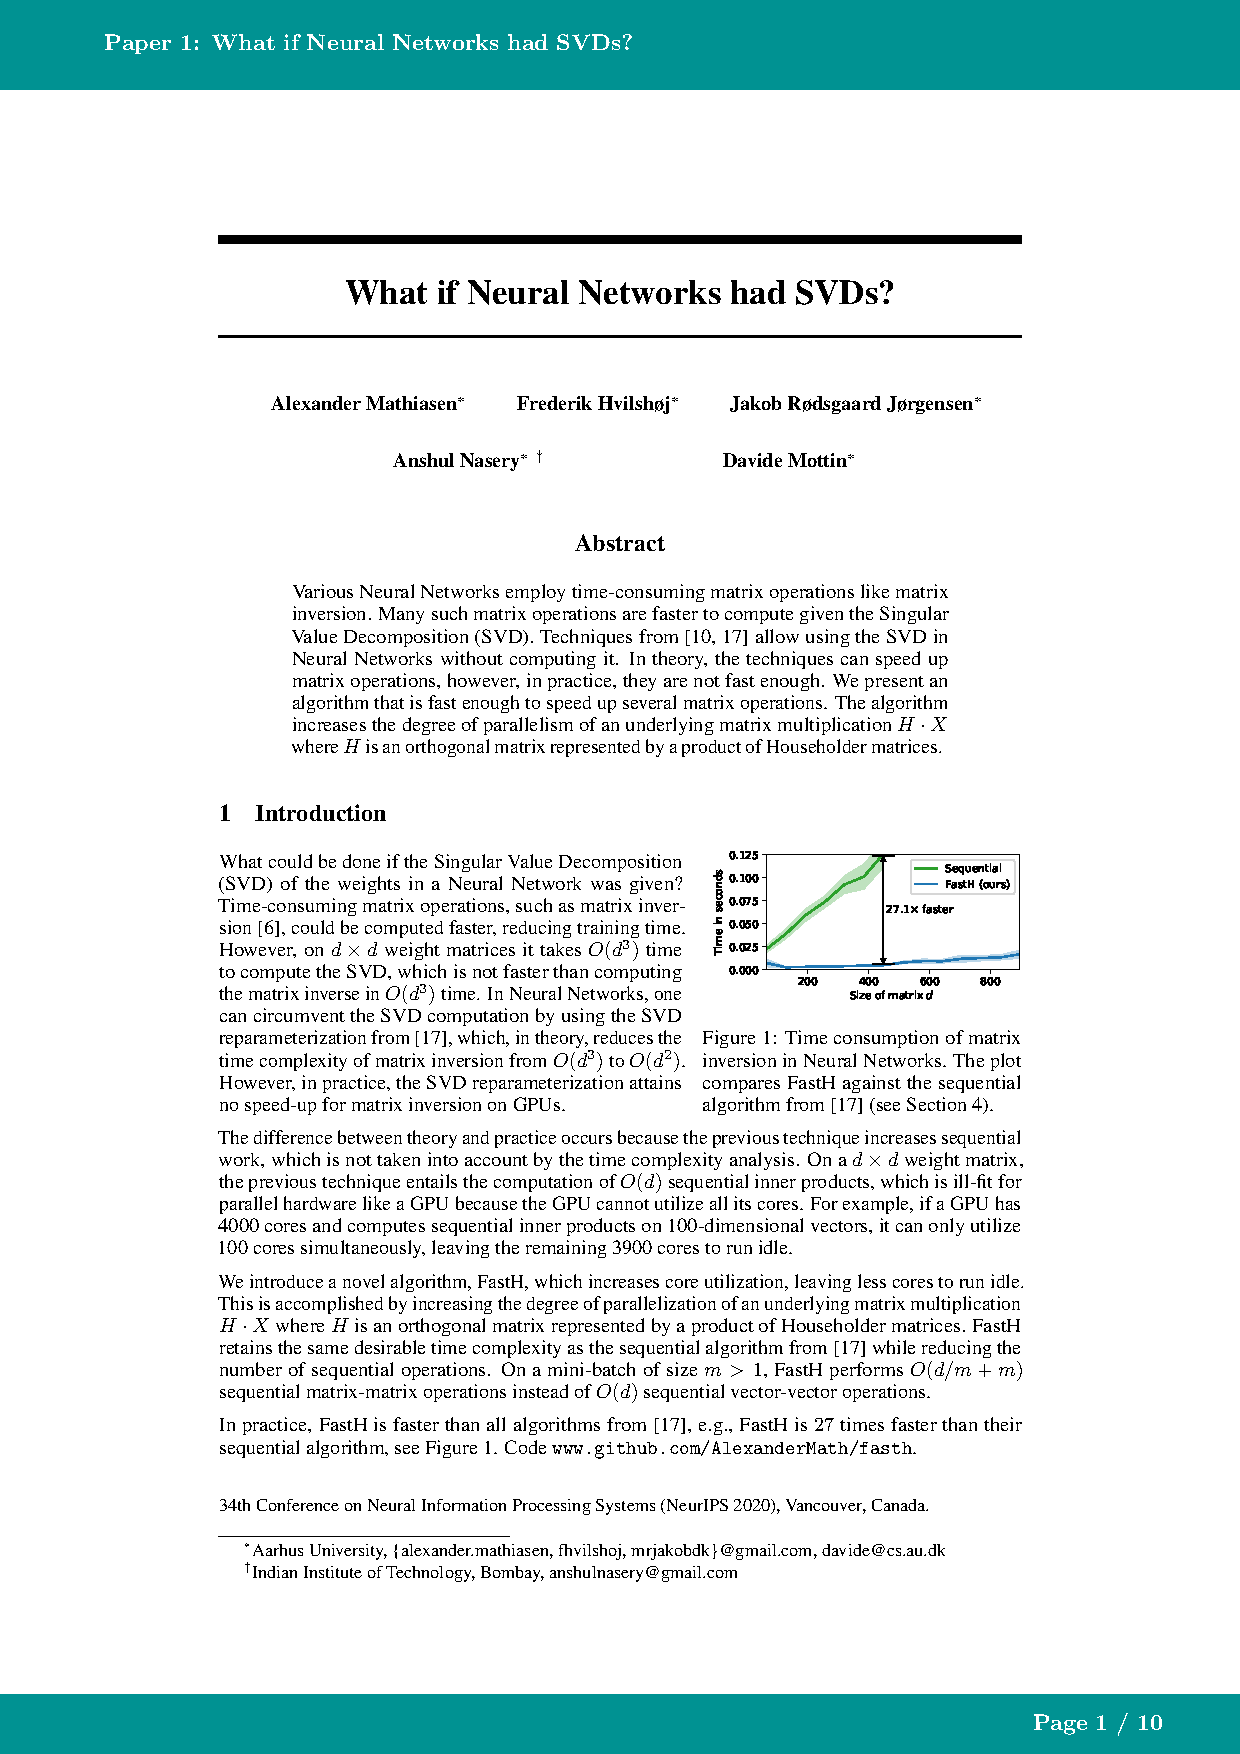
\includepdf[pages=-10]{papers/svd_w.pdf}

% FastFID
\chapter{Backpropagating through Fr\'echet Inception Distance}
\label{chap:fastfid}
\paperlabel{pap:fastfid}
\chapterprecishere{
    \textbf{Publication}: Manuscript\\
    \textbf{Author contributions:} Alexander and I made equal contributions to this paper. I participated in all parts of the project, from developing the theory to designing experiments, and writing the paper. 
}
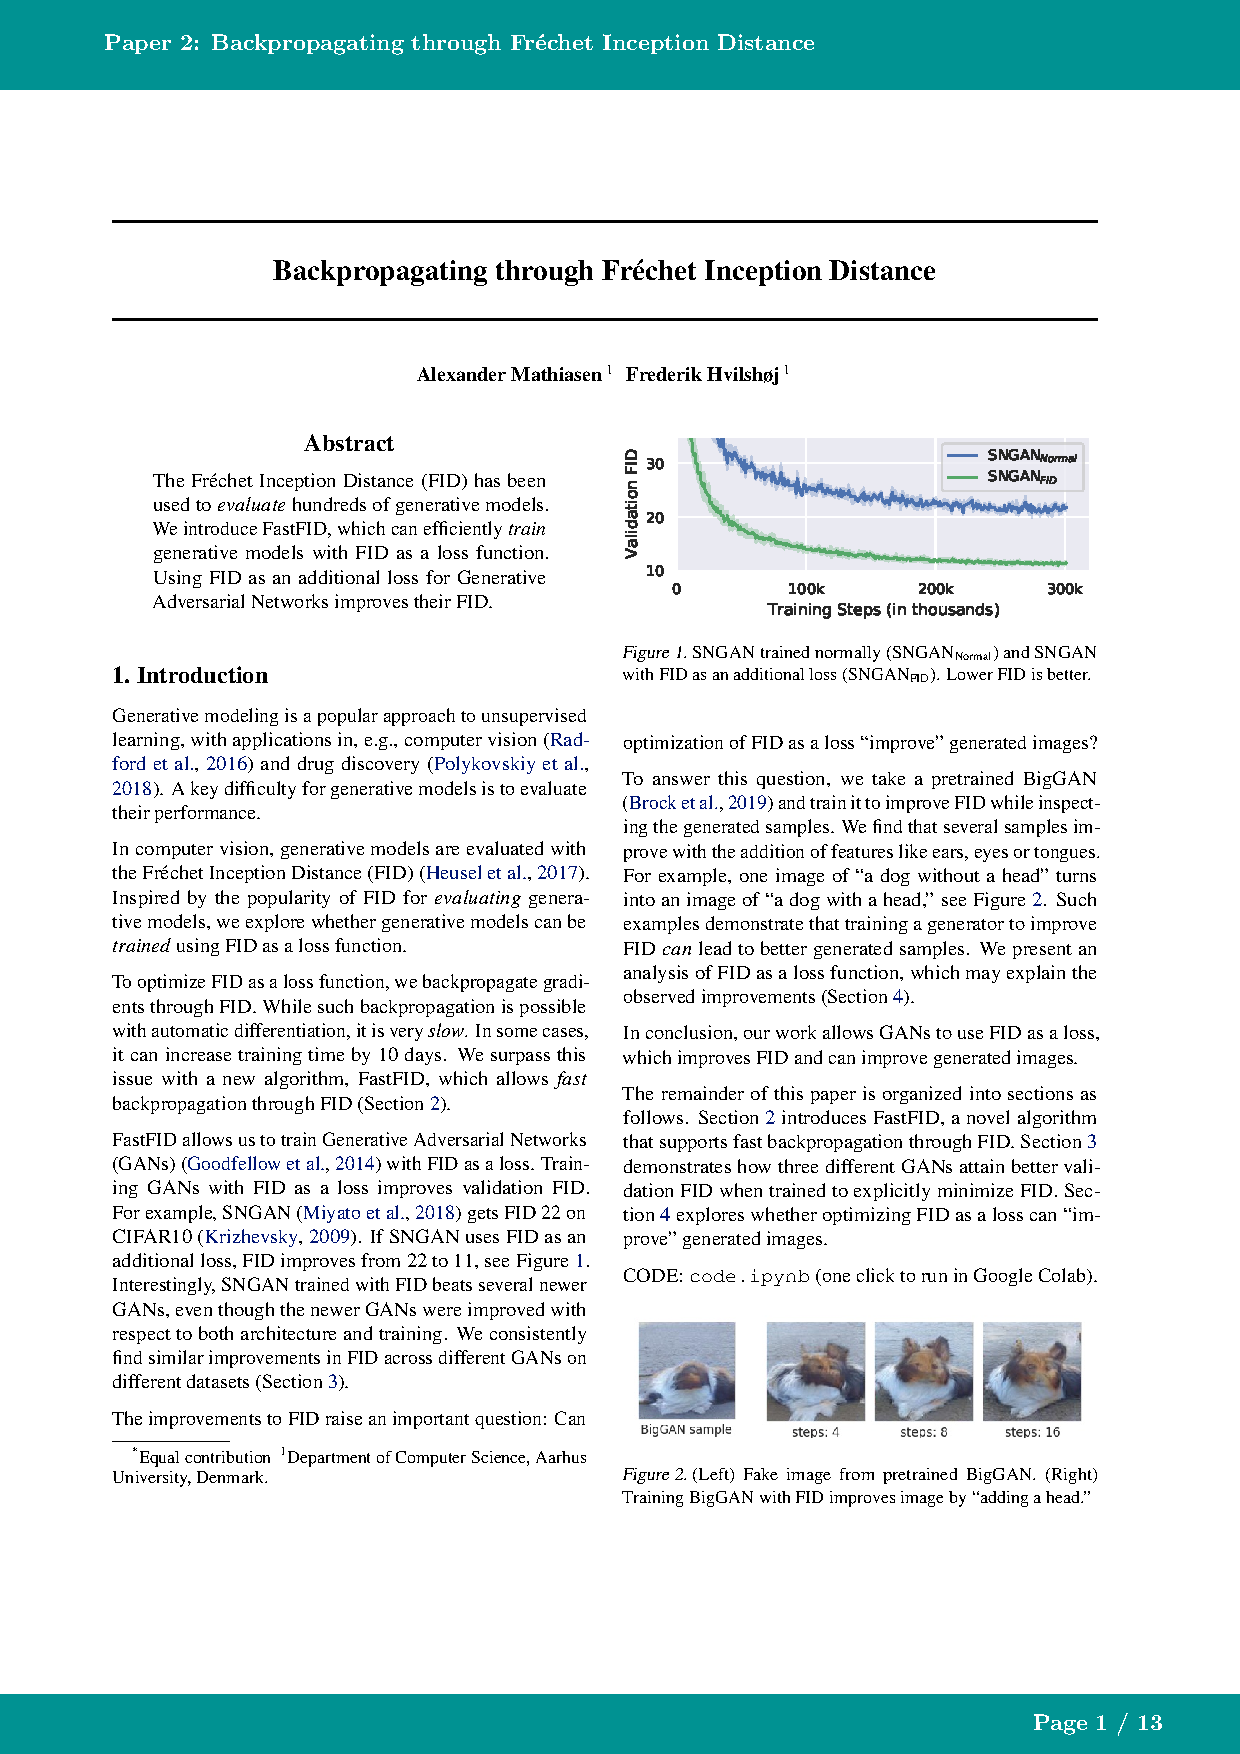
\includepdf[pages=-13]{papers/fastfid_w.pdf}

% ECINN
\chapter{ECINN: Efficient Counterfactuals from Invertible Neural Networks}
\label{chap:ecinn}
\paperlabel{pap:ecinn}
\chapterprecishere{
    \textbf{Publication}: Accepted at the British Machine Vision Conference, 2021.\\
    \textbf{Author contributions:} I was the main contributor to this paper.
}
\includepdf[pages=-19]{papers/ecinn_w.pdf}

% Evaluating counterfactuals. 
\chapter{On Quantitative Evaluations of Counterfactuals}
\label{chap:evaluation-paper}
\paperlabel{pap:evaluation}
\chapterprecishere{
    \textbf{Publication}: Manuscript\\
    \textbf{Author contributions:} I was the main contributor to this paper.
}
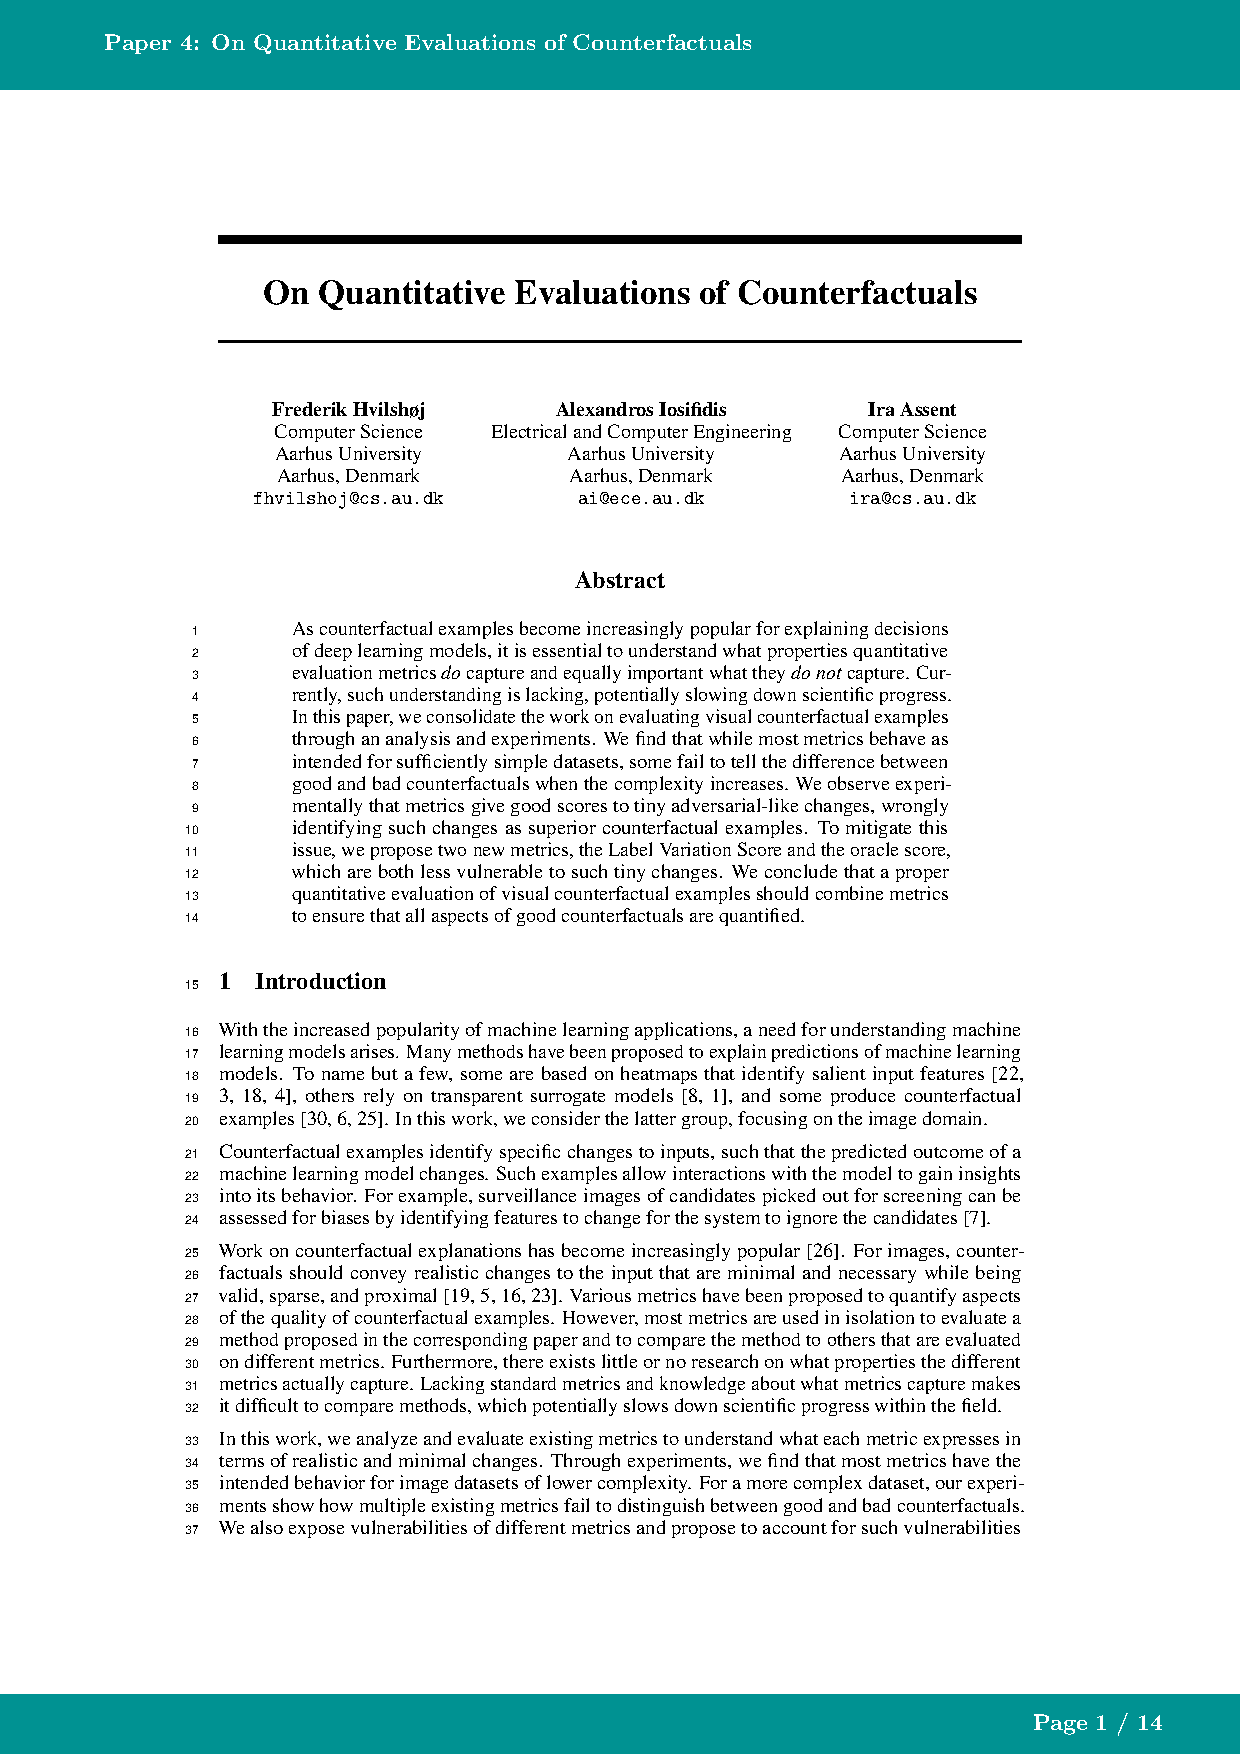
\includepdf[pages=-14]{papers/eval_w.pdf}

\backmatter

%%%%%%%%%%%%%%%%%%%%%%%%%%%%%%%%%%%%%%%%%%%%%%%%%%%%%%%%%%%%%%%%%%%%%%%%%%%%%
%% The appendix
%%%%%%%%%%%%%%%%%%%%%%%%%%%%%%%%%%%%%%%%%%%%%%%%%%%%%%%%%%%%%%%%%%%%%%%%%%%%%
% \part{Appendix}
% \appendix

%%%%%%%%%%%%%%%%%%%%%%%%%%%%%%%%%%%%%%%%%%%%%%%%%%%%%%%%%%%%%%%%%%%%%%%%%%%%%
%% The bibliography
%%%%%%%%%%%%%%%%%%%%%%%%%%%%%%%%%%%%%%%%%%%%%%%%%%%%%%%%%%%%%%%%%%%%%%%%%%%%%

\cleardoublepage
\bibliographystyle{plainnat} 
\bibliography{bibliography}

\end{document}
